\documentclass[a4paper,nobib,makeidx,justified,twoside,symmetric]{tufte-book}

\usepackage[utf8]{inputenc}
\usepackage[spanish]{babel}
\usepackage{ntheorem}
\theoremseparator{:}
\newtheorem{hyp}{Hipótesis}
\newtheorem{definition}{Definición}
\usepackage{listingsutf8}
\lstset
{
	language=[LaTeX]TeX,
	breaklines=true,
	basicstyle=\tt\scriptsize,
	keywordstyle=\color{blue},
	identifierstyle=\color{magenta},
}
\setlength{\parskip}{0.5\baselineskip}%
\setlength{\parindent}{0pt}%

\def\thetitle{Modelado de comportamiento de conductores con técnicas de Inteligencia Computacional}
\def\theauthor{Alberto Díaz Álvarez}
\def\thedate{\today}

\hypersetup{colorlinks}
\title{\thetitle}
\author[\theauthor]{\theauthor}
\authortitle{Máster en Ciencias y Tecnologías de la Computación}
\department{Departamento de Inteligencia Artificial}
\school{Escuela Técnica Superior de Ingenieros Informáticos}
\university{Universidad Politécnica de Madrid}
\advisor{Dr. Francisco Serradilla García}
\advisortitle{Doctor en Inteligencia Artificial}

\IfFileExists{bergamo.sty}{\usepackage[osf]{bergamo}}{} % Bembo
\IfFileExists{chantill.sty}{\usepackage{chantill}}{} % Gill Sans

%\usepackage{microtype}
\usepackage{booktabs}
\usepackage{graphicx}

\setkeys{Gin}{width=\linewidth,totalheight=\textheight,keepaspectratio}
\graphicspath{{images/}}

\usepackage{fancyvrb}
\fvset{fontsize=\normalsize}

\newcommand{\hangp}[1]{\makebox[0pt][r]{(}#1\makebox[0pt][l]{)}}

\newcommand{\hangstar}{\makebox[0pt][l]{*}}

\usepackage{xspace}

% Prints the month name (e.g., January) and the year (e.g., 2008)
\newcommand{\monthyear}{%
  \ifcase\month\or January\or February\or March\or April\or May\or June\or
  July\or August\or September\or October\or November\or
  December\fi\space\number\year
}

% Inserts a blank page
\newcommand{\blankpage}{\newpage\hbox{}\thispagestyle{empty}\newpage}

\usepackage{units}

% Typesets the font size, leading, and measure in the form of 10/12x26 pc.
\newcommand{\measure}[3]{#1/#2$\times$\unit[#3]{pc}}

% Macros for typesetting the documentation
\newcommand{\hlred}[1]{\textcolor{Maroon}{#1}}% prints in red
\newcommand{\hangleft}[1]{\makebox[0pt][r]{#1}}
\newcommand{\hairsp}{\hspace{1pt}}% hair space
\newcommand{\hquad}{\hskip0.5em\relax}% half quad space
\newcommand{\TODO}{\textcolor{red}{\bf TODO!}\xspace}
\providecommand{\XeLaTeX}{X\lower.5ex\hbox{\kern-0.15em\reflectbox{E}}\kern-0.1em\LaTeX}
\newcommand{\tXeLaTeX}{\XeLaTeX\index{XeLaTeX@\protect\XeLaTeX}}
% \index{\texttt{\textbackslash xyz}@\hangleft{\texttt{\textbackslash}}\texttt{xyz}}
\newcommand{\tuftebs}{\symbol{'134}}% a backslash in tt type in OT1/T1
\newcommand{\doccmdnoindex}[2][]{\texttt{\tuftebs#2}}% command name -- adds backslash automatically (and doesn't add cmd to the index)
\newcommand{\doccmddef}[2][]{%
  \hlred{\texttt{\tuftebs#2}}\label{cmd:#2}%
  \ifthenelse{\isempty{#1}}%
    {% add the command to the index
      \index{#2 command@\protect\hangleft{\texttt{\tuftebs}}\texttt{#2}}% command name
    }%
    {% add the command and package to the index
      \index{#2 command@\protect\hangleft{\texttt{\tuftebs}}\texttt{#2} (\texttt{#1} package)}% command name
      \index{#1 package@\texttt{#1} package}\index{packages!#1@\texttt{#1}}% package name
    }%
}% command name -- adds backslash automatically
\newcommand{\doccmd}[2][]{%
  \texttt{\tuftebs#2}%
  \ifthenelse{\isempty{#1}}%
    {% add the command to the index
      \index{#2 command@\protect\hangleft{\texttt{\tuftebs}}\texttt{#2}}% command name
    }%
    {% add the command and package to the index
      \index{#2 command@\protect\hangleft{\texttt{\tuftebs}}\texttt{#2} (\texttt{#1} package)}% command name
      \index{#1 package@\texttt{#1} package}\index{packages!#1@\texttt{#1}}% package name
    }%
}% command name -- adds backslash automatically
\newcommand{\docopt}[1]{\ensuremath{\langle}\textrm{\textit{#1}}\ensuremath{\rangle}}% optional command argument
\newcommand{\docarg}[1]{\textrm{\textit{#1}}}% (required) command argument
\newenvironment{docspec}{\begin{quotation}\ttfamily\parskip0pt\parindent0pt\ignorespaces}{\end{quotation}}% command specification environment
\newcommand{\docenv}[1]{\texttt{#1}\index{#1 environment@\texttt{#1} environment}\index{environments!#1@\texttt{#1}}}% environment name
\newcommand{\docenvdef}[1]{\hlred{\texttt{#1}}\label{env:#1}\index{#1 environment@\texttt{#1} environment}\index{environments!#1@\texttt{#1}}}% environment name
\newcommand{\docpkg}[1]{\texttt{#1}\index{#1 package@\texttt{#1} package}\index{packages!#1@\texttt{#1}}}% package name
\newcommand{\doccls}[1]{\texttt{#1}}% document class name
\newcommand{\docclsopt}[1]{\texttt{#1}\index{#1 class option@\texttt{#1} class option}\index{class options!#1@\texttt{#1}}}% document class option name
\newcommand{\docclsoptdef}[1]{\hlred{\texttt{#1}}\label{clsopt:#1}\index{#1 class option@\texttt{#1} class option}\index{class options!#1@\texttt{#1}}}% document class option name defined
\newcommand{\docmsg}[2]{\bigskip\begin{fullwidth}\noindent\ttfamily#1\end{fullwidth}\medskip\par\noindent#2}
\newcommand{\docfilehook}[2]{\texttt{#1}\index{file hooks!#2}\index{#1@\texttt{#1}}}
\newcommand{\doccounter}[1]{\texttt{#1}\index{#1 counter@\texttt{#1} counter}}

\usepackage{marginfix}
\usepackage{mparhack}

\usepackage[acronym,shortcuts]{glossaries}

\makeglossaries

\glsaddkey
{longsp}% key
{}% default value
{\glsentrylongsp}% new command analogous to \glsentrylong
{\Glsentrylongsp}% new command analogous to \Glsentrylong
{\acrlongsp}% new command analogous to \acrlong
{\Acrlongsp}% new command analogous to \Acrlong
{\ACRlongsp}% new command analogous to \ACRlong

% Add new key for plural long Spanish form:
\glsaddkey
{longplsp}% key
{}% default value
{\glsentrylongplsp}% new command analogous to \glsentrylongpl
{\Glsentrylongplsp}% new command analogous to \Glsentrylongpl
{\acrlongplsp}% new command analogous to \acrlongpl
{\Acrlongplsp}% new command analogous to \Acrlongpl
{\ACRlongplsp}% new command analogous to \ACRlongpl

% Provide conditional to test if longsp/longplsp has been set
\newcommand*{\glsifhaslongsp}[3]{%
	\ifcsempty{glo@#1@longsp}{#3}{#2}%
}
\newcommand*{\glsifhaslongplsp}[3]{%
	\ifcsempty{glo@#1@longplsp}{#3}{#2}%
}

% Define new acronym style:

\newacronymstyle{spanish}
{% base the display style on 'long-short'
	\GlsUseAcrEntryDispStyle{long-short}%
}%
{% base the definitions on 'long-short'
	\GlsUseAcrStyleDefs{long-short}%  
	% Make some custom modifications for the first use display.
	% Singular, no case change:
	\renewcommand*{\genacrfullformat}[2]{%
		\glsifhaslongsp{##1}%
		{% has Spanish version:
			\glsentrylongsp{##1}##2\space
			(\firstacronymfont{\glsentryshort{##1}}, \glsentrylong{##1})%
		}%
		{%
			\glsentrylong{##1}##2\space
			(\firstacronymfont{\glsentryshort{##1}})%
		}%
	}%
	% Singular, first letter upper case:
	\renewcommand*{\Genacrfullformat}[2]{%
		\glsifhaslongsp{##1}%
		{% has Spanish version:
			\Glsentrylongsp{##1}##2\space
			(\firstacronymfont{\glsentryshort{##1}}, \glsentrylong{##1})%
		}%
		{%
			\Glsentrylong{##1}##2\space
			(\firstacronymfont{\glsentryshort{##1}})%
		}%
	}%
	% Plural, no case change:
	\renewcommand*{\genplacrfullformat}[2]{%
		\glsifhaslongplsp{##1}%
		{% has Spanish version:
			\glsentrylongplsp{##1}##2\space
			(\firstacronymfont{\glsentryshortpl{##1}}, \glsentrylongpl{##1})%
		}%
		{%
			\glsentrylongpl{##1}##2\space
			(\firstacronymfont{\glsentryshortpl{##1}})%
		}%
	}%
	% Plural, first letter upper case:
	\renewcommand*{\Genplacrfullformat}[2]{%
		\glsifhaslongplsp{##1}%
		{% has Spanish version:
			\Glsentrylongplsp{##1}##2\space
			(\firstacronymfont{\glsentryshortpl{##1}}, \glsentrylongpl{##1})%
		}%
		{%
			\Glsentrylongpl{##1}##2\space
			(\firstacronymfont{\glsentryshortpl{##1}})%
		}%
	}%
}

% switch to the new style:
\setacronymstyle{spanish}

% Define a new glossary style that checks for the existence of
% the longsp field.
\newglossarystyle{listsp}{%
	\setglossarystyle{list}% base style on the list style
	\renewcommand*{\glossentry}[2]{%
		\item[\glsentryitem{##1}%
		\glstarget{##1}{\glossentryname{##1}}]
		\glossentrydesc{##1}%
		\glsifhaslongsp{##1}{\space(\glsentrylongsp{##1})}{}%
		\glspostdescription\space ##2}%
}


% Aquí todas las definiciones y acrónimos
\newacronym[longsp=Estudio Naturalista de Conducción,longplsp=Estudios Naturalistas de Conducción,longplural=Naturalistic driving studies]{nds}{NDS}{Naturalistic driving study}
\newacronym[longsp=Reconocimento el Entorno Intravehicular,longplsp=Reconocimientos del Entorno Intravehiculares,longplural=Intra-vehicular Context Awarenesses]{ivca}{IvCA}{Intra-vehicular Context Awareness}
\newacronym[longsp=Sistema Avanzado de Ayuda a la Conducción,longplsp=Sistemas Avanzados de ayuda a la Conducción,longplural=Advanced Driver Assistance Systems]{adas}{ADAS}{Advanced Driver Assistance System}
\newacronym{torcs}{TORCS}{The Simulated Car Racing Championship}
\newacronym[longsp=Procesamiento Complejo de Eventos,longplsp=Procesamientos Complejos de Eventos,longplural=Complex Event Processings]{cep}{CEP}{Complex Event Processing}
\newacronym[longsp=Inteligencia Artificial,longplsp=Inteligencias Artificiales]{ai}{AI}{Artificial Intelligence}
\newacronym[longsp=Inteligencia Computacional,longplsp=Inteligencias Computacionales,longplural=Computational Intelligences]{ci}{CI}{Inteligencia Computacional}
\newacronym[longsp=Sistema Inteligente de Transporte,longplsp=Sistemas Inteligentes de Transporte,longplural=Intelligent Transport Systems]{its}{ITS}{Intelligent Transport System}
\newacronym[longsp=Sistema Multi-Agente,longplsp=Sistemas Multi-Agentes,longplural=Multi-Agent Systems]{mas}{MAS}{Multi-Agent System}

\makeglossaries

\usepackage{smartdiagram}
\usepackage[caption=false]{subfig}

\usepackage{tikz}
\usetikzlibrary{matrix,arrows,arrows.meta,shapes,trees,mindmap}
\usepackage{smartdiagram}

\usepackage{pgfplots}

\usepackage{todonotes}

\usepackage{pifont}
\newcommand{\yep}{\textcolor{ForestGreen}{\ding{51}}}
\newcommand{\nop}{\textcolor{Red}{\ding{55}}}
\newcommand{\na}{\textcolor{Dandelion}{--}}
 
\usepackage[
type={CC},
modifier={by-sa},
version={3.0},
]{doclicense}

%\setcounter{secnumdepth}{2}
\titleformat{\chapter}%
[display]% shape
{\relax\ifthenelse{\NOT\boolean{@tufte@symmetric}}{\begin{fullwidth}}{}}% format applied to label+text
	{\itshape\huge\chaptertitlename~\thechapter}% label
	{0pt}% horizontal separation between label and title body
	{\huge\rmfamily\itshape}% before the title body
	[\ifthenelse{\NOT\boolean{@tufte@symmetric}}{\end{fullwidth}}{}]% after the title body

\usepackage{imakeidx}
\makeindex
\newcommand\idx[1]{#1\index{#1}}

% Para definición de ecuaciones por partes (dos partes)
\newcommand{\twopartf}[4]
{
	\left\{
	\begin{array}{ll}
		#1 & \mbox{si } #2 \\
		#3 & \mbox{si } #4
	\end{array}
	\right.
}

\usepackage{morefloats}

\begin{document}

\hyphenpenalty=10

\frontmatter
\maketitle
\cleardoublepage
\begin{fullwidth}
~\vfill
\thispagestyle{empty}
\setlength{\parindent}{0pt}
\setlength{\parskip}{\baselineskip}
\theauthor

\par{
	\textit{\thetitle}\\*
	Tesis doctoral, \thedate\\*
	Revisores: Rev1, Rev2 y Rev3\\*
	Dirección: \thanklessadvisorone, \thanklessadvisortwo
	}

\par{
	\textbf{Instituto Universitario de Investigación del Automóvil}\\*
	Universidad Politécnica de Madrid\\*
	Campus Sur UPM, Carretera de Valencia (A-3), km7\\*
	28031 Madrid
}

\par{
	\doclicenseThis
}

\end{fullwidth}

\cleardoublepage
~\vfill
\thispagestyle{empty}
\begin{doublespace}
\noindent\fontsize{16}{20}\selectfont\itshape
\nohyphenation .
\end{doublespace}
\vfill
\vfill


\cleardoublepage

\tableofcontents
\printglossaries
\listoffigures
\listoftables

\mainmatter
\part{Introducción}
\chapter{Introducción}
\label{ch:intro}

Es un hecho que la \ac{ai} en general (y la \ac{ci} en particular) como área de conocimiento ha experimentado un creciente interés en los últimos años. Esto no siempre ha sido así, ya que después de un nacimiento muy esperanzador, con mucho optimismo, le siguieron unas épocas de apenas avance (ver cuadro~\ref{tbl:ai-timeline}). Sin embargo, en la actualidad es muy difícil encontrar un campo que no se beneficie directamente de sus técnicas.

\begin{table}
	\centering
	\begin{minipage}[t]{\linewidth}
		\newcommand\ytl[2]{
			\parbox[b]{1cm}{\hfill{\color{cyan}\bfseries\sffamily #1}~$\cdots$~}
			\parbox[c]{3.8cm}{\vspace{7pt}\raggedright\sffamily #2.\\[0pt]}\\[0pt]}
		\color{gray}

		\ytl{1956}{Conferencia de Dartmouth. Nace el campo de la \ac{ai}. Se destinan muchos recursos debido al potencial del nuevo campo.}
		\ytl{1974}{No llegan los resultados esperados. Se suspenden financiaciones y se deja de investigar en muchas áreas (\textit{AI Winter})}
		\ytl{1980}{Aparecen los sistemas expertos. Muy prometedores. Acaparan la práctica totalidad de la investigación en \ac{ai}.}
		\ytl{1987}{De nuevo los resultados no son lo esperado y vuelve a dinsminuir el trabajo en \ac{ai}.}
		\ytl{1990}{La mejora de las prestaciones, la ubicuidad de los ordenadores y nuevos conceptos (e.g. agentes) hacen que la investigación en el área vuelva a crecer. Se replantea el concepto de \ac{ai}.}
		\ytl{2000}{Se retoman investigaciones relacionadas con el aprendizaje profundo. Aumenta la investigación en el área de las redes neuronales y redes bayesianas.}
		\ytl{2006}{Conferencia de Dartmouth. Se analizan los avances y se debate sobre la \ac{ai} a 50 años vista. Crece la expectación y el interés en el campo}
		\ytl{2007}{Crece el interés en el aprendizaje automático debido a los resultados obtenidos y el aumento de las fuentes de datos}
		\bigskip
		\caption{Línea temporal de los principales hitos en la \glsentrytext{ai}. Actualmente la \glsentrytext{ai} está ofreciendo resultados muy prometedores áreas como la conducción autónoma, el procesamiento del lenguaje natural o el análisis de sentimiento entre muchos otros.\TODO{La he movido del margen porque no cabía en tamaño b5. Hay que recolocarla por aquí.}}
		\label{tbl:ai-timeline}
	\end{minipage}
\end{table}

Una de sus razones es su caracter multidisciplinar ya que, si bien se la define como área perteneciente al campo de la informática, es transversal a muy diferentes campos, como pueden ser por ejemplo la biología, neurología o la psicología, entre otros.

Dentro del área de la \acrlongsp{ai} es común diferenciar dos tipos de aproximaciones a la hora de hablar de cómo representar el conocimiento: la \textbf{\acrlongsp{ai} clásica}, que postula que el conocimiento como tal se puede reducir a un conjunto de símbolos con operadores para su manipulación, y la \textbf{\acrlongsp{ci}}, que defiende que al conocimiento se llega a través del aprendizaje, y que basa sus esfuerzos en la simulación de elementos de bajo nivel que subyacen a los comportamientos inteligentes esperando que el conocimiento \enquote{emerja} de éstos.

El límite entre ambos conjuntos no está perfectamente definido, máxime si tenemos en cuenta las diferentes terminologías existentes, las sinergias entre distintas técnicas dentro del área y los diferentes puntos de vista sobre éstas por parte de los autores. Sin embargo, una de las principales diferencias de ambos paradigmas es el punto de vista a la hora de solucionar problemas, siendo la aproximación \textbf{top-down} la usada en problemas de \acrshort{ai} clásica y la \textbf{bottom-up} la típica usada en la \acrshort{ci}. Revisaremos las diferencias entre conceptos de diferentes autores en el capítulo \ref{ch:sota-ci}\sidenote{Una aproximación \textit{top-down} a los problemas funciona definiendo primero el algoritmos que resuelve el problema para posteriormente ejecutarlo y llegar así a la solución exacta. Por otro lado, una aproximación \textit{bottom-up} el algoritmo de resolución no se programa, sino que se aprende, llegando él sólo a soluciones no necesariamente exactas pero sí lo suficientemente buenas para ser aceptadas.}.

Uno de los campos de aplicación es el de los \acp{its}. Éstos se definen como un conjunto de aplicaciones orientadas a gestionar el transporte en todos sus aspectos y granularidades (e.g. conducción eficiente, diseño de automóviles, gestión del tráfico o señalización en redes de carreteras) para hacerlos más eficientes y seguros. El interés es tal que en el año 2010 se publicó la directiva 2010/40/UE (ver \cite{parliament2010directive}) donde se estableció el marco de implantación de los ITS en la Unión Europea\footnote{En esta directiva, los ITS se definen como \textit{aplicaciones avanzadas que, sin incluir la inteligencia como tal, proporcionan servicios innovadores en relación con los diferentes modos de transporte y la gestión del tráfico y permiten a los distintos usuarios estar mejor informados y hacer un uso más seguro, más coordinado y «más inteligente» de las redes de transporte.}}.

En el caso concreto del comportamiento al volante, es interesante la evaluación de los conductores para conocer su manera de actuar en determinados escenarios, y poder extraer información de éstos que nos permitan, por ejemplo, detectar qué factores pueden afectar más o menos a determinados indicadores (e.g. el consumo estimado para una ruta en concreto). Sin embargo, la evaluación en distintos escenarios puede no ser interesante debido a limitaciones existentes, como pueden ser, por ejemplo, el tiempo, el dinero o la peligrosidad del escenario.

Los simuladores de tráfico son una solución para muchas de estas limitaciones, pero suelen basar su funcionamiento en conductores y vehículos (normalmente concebidos como una única entidad) basándose en modelos de conductor que responden a funciones más o menos complejas, además con pocas o ningunas opciones de personalización. Esto provoca que dichos modelos se adapten poco al modelo de un conductor en concreto.

Esta tesis pretende explorar el tema de la generación de modelos de conductor para simuladores que respondan al comportamiento de conductores reales usando, para ello, técnicas pertenecientes al campo de la \ac{ci}.

Concretamente pretende desarrollar un método para el análisis de la eficiencia de los conductores realizando, para ello, un modelo del perfil de conducción a partir de técnicas de la \ac{ci} y aplicándolo a un entorno de simulación basado en \Acp{mas}. Así, una vez configurado el entorno, se podrán estudiar aspectos generales como la evolución del tráfico con determinados perfiles o particulares como el estilo de conducción o el impacto de los sistemas de asistencia.

\section{Motivación}

Los conceptos introducidos al comienzo del capítulo obedecen a una \textit{necesidad} (aquí como eufemismo de problema) de la sociedad en la que vivimos, y que afecta tanto a nuestra generación como afectará a las venideras: la eficiencia en la conducción. Dado que es imprescindible saber que existe un problema para arreglarlo, nada mejor que puntualizar algunos hechos de sobra conocidos:

\begin{itemize}
	\item En el año 2014, el número de vehículos a nivel mundial asciende a más de $1.200$ millones, con una tendencia creciente \cite{oica2014motrate}. Reducir en un pequeño porcentaje el consumo durante la conducción evita la emisión de toneladas de gases considerados nocivos para el medio ambiente y el ser humano\footnote{Uno puede argumentar que el parque automovilístico se recicla con nuevos vehículos eléctricos categorizados \enquote{de consumo 0}. La triste realidad es que estos vehículos consumen la electricidad generada actualmente de una mayoría de centrales de combustibles fósiles y nucleares. Además, mientras que en países desarrollados el crecimiento ha sido en torno al 4-7\%, en países subdesarrollados, donde no existe aun infraestructura para la recarga de vehículos eléctricos, dicho crecimiento ha superado el 120\%.}.
	\item Debemos abandonar los combustibles fósiles antes de que éstos nos abandonen a nosotros. Si bien es cierto que existen diferentes puntos de vista acerca de cuándo se agotarán las reservas de petróleo, también lo es que los combustibles fósiles son recursos \textbf{finitos}. Lo más probable es que no se llegue a agotar debido a la ley de la oferta y la demanda, pero hay que recordar que el petróleo se usa como base para la producción de otros muchos tipos de productos, como por ejemplo la vaselina, el asfalto o los plásticos.
	\item Independientemente del momento en el que se agoten los recursos, hay que hacer notar que la emisión de gases está correlacionada con el aumento de la temperatura del planeta, hecho que se ilustra en la figura~\ref{fig:co2-global-warm-correlation}. De seguir con el ritmo de consumo actual, se teme llegar a un punto de no retorno con consecuencias catastróficas para la vida en el planeta.

\begin{marginfigure}
	\centering
	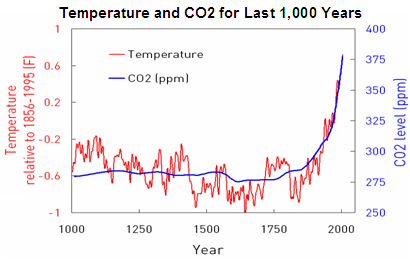
\includegraphics{images/co2-global-warm-correlation}
	\caption{Desde el comienzo de la revolución industrial, el uso masivo de combustibles fósiles y el crecimiento de la población propició un aumento desproporcionado de $CO_2$ a la atmósfera, tendencia que sigue en aumento aún con la (lenta) adopción del vehículo eléctrico. La gráfica muestra cómo ambos valores parecen estar correlacionados. Fuente: Environmental Defense Fund (\url{edf.org}).}
	\label{fig:co2-global-warm-correlation}
\end{marginfigure}

	\item Algo más cercano en el tiempo. La conducción eficiente afecta directamente a factores correlacionados con el número de accidentes de tráfico. Un factor de sobra conocido es el de la velocidad, factor relacionado no sólo con el número sino con la gravedad de los accidentes\cite{imprialou2016re}. Otros indicadores son las aceleraciones, deceleraciones y maniobras de cambio de dirección, cuya frecuencia es inversamente proporcional a la eficiencia en la conducción y directamente proporcional a la agresividad, falta de seguridad y accidentes (\cite{dingus2006100} y \cite{lerner2010exploration}).
\end{itemize}

Estos hechos son solo algunos que ponen de manifiesto la necesidad de centrarse en el problema de cómo hacer de la conducción una actividad más eficiente y segura.

La \textbf{conducción eficiente} o \textit{eco-driving} es definida como la aplicación de una serie de reglas de conducción con el objetivo de reducir el consumo de combustible, independientemente del tipo (e.g. electricidad, gasolina, gas natural, \ldots).

Ser capaces de identificar o al menos estimar qué conductores son considerados como no eficientes es importante debido a que, de esta manera, se pueden identificar los hábitos recurrentes en este tipo de perfil y adecuar la formación para eliminar dichos hábitos. Más aún teniendo en cuenta la relación existente entre la peligrosidad y algunas conductas agresivas. Un ejemplo donde la identificación de perfiles no eficientes pueden tener impacto claro económico y social es el de las empresas cuya actividad se basa en el transporte de mercancías o de personas.

Sin embargo, identificar la conducta de un conductor no es fácil, dado que su comportamiento se ve condicionado por numerosos factores como el estado de la ruta, el del tráfico o el estado físico o anímico. Además, la ambigüedad de las situaciones dificulta todavía más la identificación. Por ejemplo, un conductor puede ser clasificado en un momento como agresivo o no eficiente en una situación únicamente porque su comportamiento ha sido condicionado por las malas reacciones por parte de los demás conductores.

El análisis de todos los posibles casos es una tarea prácticamente imposible. Por ello, las simulaciones pueden dar una estimación de los posibles resultados de un estudio en el mundo real. Las simulaciones con \acp{mas} representan a los conductores como agentes permitiendo la evaluación del comportamiento tanto individual como general del sistema en base a sus individuos a través de iteraciones discretas de tiempo.

Si dichos agentes son obtenidos mediante la modelización de conductores a partir de sus datos reales, su comportamiento en la simulación podría ser considerado como fuente de datos para condiciones de tráfico y/o rutas no contempladas en el mundo real. De esta forma, se dispondría de un marco de trabajo para la comparación de diferentes conductores sin necesidad de exponerlos a todos y cada uno de los posibles eventos posibles. También sería factible evaluar sistemas de asistencia evitando los problemas de no comparabilidad de condiciones del entorno entre pruebas.

Demostrar que la evaluación de un modelo del conductor en entornos simulados es equivalente a la evaluación de conductores en entornos reales implica que se pueden comparar dos conductores usando un criterio objetivo, es decir, sin depender del estado del resto de factores a la hora de realizar la prueba de campo. Dicho de otro modo, implicaría que es posible comparar la eficiencia de dos conductores independientemente del estado del tráfico e, incluso, sobre rutas diferentes.

\section{Objetivos}
\label{ch:intro:objectives}

El objetivo de esta tesis doctoral es la de demostrar la hipótesis~\ref{hyp:hypothesis-1}, quedando dicha demostración dentro de los límites impuestos por los supuestos y restricciones indicados más adelante.

\begin{hyp}[H\ref{hyp:hypothesis-1}] \label{hyp:hypothesis-1}
	La aplicación de técnicas pertenecientes al campo de la \ac{ci} con datos extraídos de un entorno de microsimulación de espacio continuo y tiempo discreto basado en sistemas multiagentes permitirá modelar, de manera fiel a la realidad, el comportamiento de conductores reales.
\end{hyp}

Por tanto, el objetivo de la tesis es el de simular el comportamiento de conductores en entornos de micro-simulación a partir de su comportamiento en entornos reales usando técnicas de \ac{ci}. Para ello se consideran los siguientes objetivos específicos:

\begin{itemize}
	\item Estudiar y aplicar técnicas de la \ac{ci} sobre el área de la conducción.
	\item Realizar un \gls{nds}\sidenote{Los \gls{nds} basan su funcionamiento en la captura masiva de datos de conducción, normalmente involucrando una gran cantidad de sensores, para analizar el comportamiento del conductor, las características del vehículo, la vía, etcétera. La cantidad de sensores y la velocidad de captura hacen que la tarea de analizar y extraer conclusiones sea una tarea prácticamemte imposible para un humano, por lo que es necesario el uso de técnicas de análisis de datos que suelen recaer en los campos de la estadística y del aprendizaje automático.} sobre conductores reales para:
	\begin{enumerate}
		\item Generar modelos personalizados de conductor a partir de los datos de conducción obtenidos.
		\item Aplicar modelos de conductores a entornos de simulación multiagente.
		\item Validar los modelos de conductor contra conductores reales.
	\end{enumerate}
	\item Estudiar la efectividad de sistemas de asistencia encaminados a mejorar la eficiencia y analizar el comportamiento de conductor.
\end{itemize}

\subsection{Supuestos}

\begin{itemize}
	\item Suponemos que el comportamiento de un conductor es el comportamiento en línea y el comportamiento de cambio de carril\footnote{Son conocidos en la literatura como \textit{car-following} y \textit{lane-changing} respectivamente. Entraremos en detalle sobre ambos conceptos en el capítulo~\nameref{ch:sota-behavior-models}}.
	\item La circulación se realizará por la dereccha.
	\item Los datos de los que extraer el comportamiento se corresponderán con lecturas realizadas durante el día, con buena visibilidad y sin lluvia.
	\item El tipo de vehículo sobre el que modelar el comportamiento será el de un utilitario.
	\item El conductor a modelar pertenecerá al grupo más representativo de conductores. Esto se corresponde con varón de $35$ a $39$ años (ver figura~\ref{fig:drivers-census}).
\end{itemize}

\begin{marginfigure}
	\resizebox {\linewidth} {!} {
	\begin{tikzpicture}
	\begin{axis}[legend style={anchor=north east},
	symbolic x coords={15--17,18--20,21--24,25--29,30--34,35--39,40--44,45--49,50--54,55--59,60--64,65--69,70--74,74+}, xtick=data, x tick label style={rotate=90,anchor=east}]
	\addlegendentry{Hombres}
	\addplot[mark=*,thick,blue] coordinates {
		(15--17,39341)
		(18--20,318037)
		(21--24,729846)
		(25--29,1097874)
		(30--34,1472038)
		(35--39,1828905)
		(40--44,1768957)
		(45--49,1688069)
		(50--54,1460193)
		(55--59,1256212)
		(60--64,1082591)
		(65--69,974768)
		(70--74,709285)
		(74+,1190514)
	};
	
	\addlegendentry{Mujeres}
	\addplot[mark=diamond*,thick,red] coordinates {
		(15--17,15697)
		(18--20,238534)
		(21--24,651961)
		(25--29,1054377)
		(30--34,1337432)
		(35--39,1568926)
		(40--44,1445740)
		(45--49,1321330)
		(50--54,1055472)
		(55--59,810168)
		(60--64,569461)
		(65--69,387158)
		(70--74,189829)
		(74+,1138945)
	};
	
	
	\end{axis}
	\end{tikzpicture}
	}
	\caption{Último censo de conductores según género segmentado por edades. Fuente: Dirección General de Tráfico (\url{dgt.es}).}
	\label{fig:drivers-census}
\end{marginfigure}
\subsection{Restricciones}

\begin{itemize}
	\item El sistema multiagente hará uso de \gls{dvu} como agentes, es decir, usando la tupla (conductor, vehículo) como un todo.
	\item La resolución máxima del modelo creado es de 1Hz.
	\item En el caso de los modelos que hacen uso de redes neuronales artificiales, no se pueden explicar las razones del comportamiento inferido.
\end{itemize}

\section{Estructura de la tesis}
\label{ch:intro:structure}

La tesis está estructurada de la siguiente manera:

En los capítulos \ref{ch:sota-traffic-simulators-and-mas}, \ref{ch:sota-ci} y \ref{ch:sota-behavior-models} se expone la revisión realizada del estado de la cuestión donde se explica en qué punto se encuentra la literatura de los temas en los que se apoya la presente tesis.

En el capítulo XXX se explica el método seguido para la confirmación de la hipótesis describiendo además las instrumentaciones, los conjuntos de datos obtenidos, las técnicas utilizadas y las aplicaciones desarrolladas.

Por último en el capítulo \ref{ch:conclusions} se exponen los resultados y las conclusiones extraídas de la tesis. Además, tras las conclusiones se indican una serie de posibles líneas futuras de trabajo consideradas interesantes tras la realización de la tesis.

\part{Estado de la cuestión}
\chapter{\glsentrylongsp{ci}}
\label{ch:sota-ci}

\begin{marginfigure}
	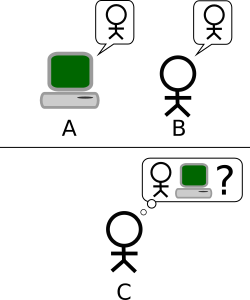
\includegraphics{turing-test}
	\caption{Ilustración del Test de Turing. Modelo propuesto para probar si una máquina es capaz de exhibir comportamiento inteligente similar al del ser humano. Hay tres participantes, dos humanos ($A$ y $C$) y una máquina ($B$), separados entre sí pero pudiendo intercambiarse mensajes de texto. $C$ envía preguntas a $A$ y $B$ sin saber quién es humano y quién es máquina y éstos le responden. Si $C$ no es capaz de identificar qué participante es la máquina, se puede concluir que la máquina es inteligente. Fuente: Hugo Férée, via Wikimedia Commons.}
	\label{fig:turing-test}
\end{marginfigure}

El comportamiento de un individuo en un entorno se ve influenciado por una infinidad de variables. Identificar las relaciones entre éstas es en la mayoría de las ocasiones una tarea que va de lo muy difícil a lo imposible, más aún si añadimos que éstas son muy numerosas y pueden llegar a ser imposibles de cuantificar o incluso de detectar.

La \ac{ci} engloba un conjunto de técnicas que facilitan enormemente estas tareas. En este capítulo se ofrece una perspectiva de la literatura actual sobre las técnicas de la \gls{ci} que son de interés para esta tesis. Introduciremos el concepto y las nociones de \enquote{agente} y de \enquote{aprendizaje} para posteriormente introducir algunas de las técnicas utilizadas dentro del área. Por último, desarrollaremos las tres técnicas principales sobre las que reposa el trabajo teórico de esta tesis: \glsentrylongplsp{ann}, \glsentrylongsp{fl} y \glsentrylongsp{cev}.

\section{\glsentrylongsp{ai} vs. \glsentrylongsp{ci}}

¿Qué es la \ac{ci}? Para entender el significado de éste término tenemos que entender cómo ha evolucionado el término \ac{ai} a lo largo de los años.

El primer concepto a introducir es el de \enquote{conexionismo}. Se puede considerar a Santiago Ramón y Cajal como principal precursor de esta idea por sus trabajos acerca de la estructura de las neuronas y sus conexiónes (e.g. \cite{y1888estructura} y~\cite{ramon1904textura}). Otros prefieren citar el trabajo \textit{\enquote{A logical calculus of the ideas immanent in nervous activity}} (\cite{McCulloch1943}) sobre \glspl{ann} o \textit{\enquote{The organization of behavior}} (\cite{hebb19680}) acerca de la teoría del aprendizaje como primeros trabajos en este tema. Independientemente de su origen, el conexionismo postula que la mente y el conocimiento surgen de redes formadas por unidades sencillas interconectadas (i.e. neuronas).

\begin{marginfigure}
	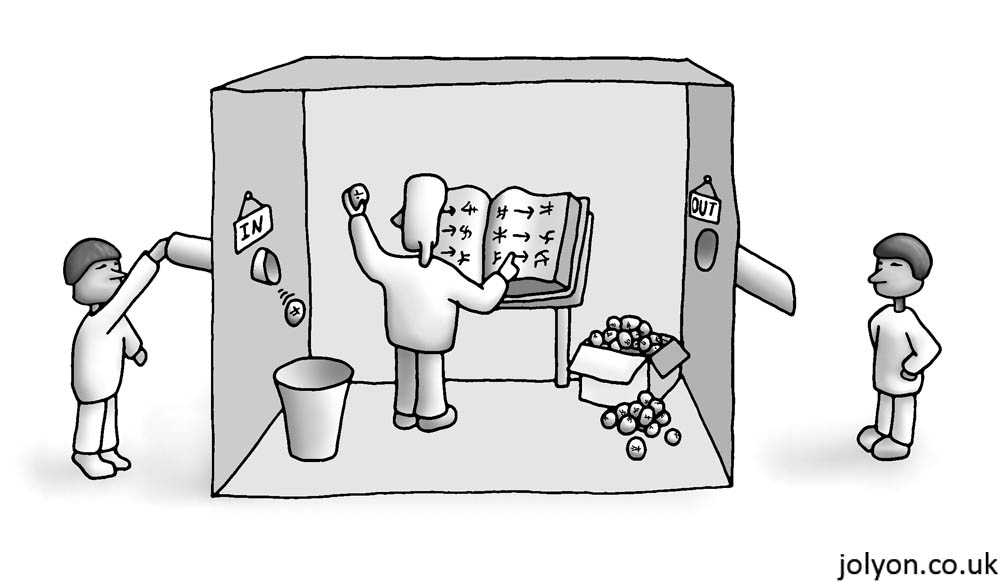
\includegraphics{chinese-room}
	\caption{\enquote{La habitación china} es un experimento mental  propuesto por John Searle que parte de un Test de Turing donde la máquina ha aprendido a hablar chino. Ésta es reemplazada por una persona que no sabe nada del idioma pero que va equipada con manual de correspondencias (ideograma de entrada $\rightarrow$ ideograma de salida). Cuando una persona le manda mensajes en chino, esta otra responde. ¿Podemos decir que dicha persona sabe chino? Evidentemente no. Pero entonces, ¿cómo podemos asegurar que la máquina reemplazada ha \enquote{aprendido} chino?. Autor: Jolyon Troscianko (http://www.jolyon.co.uk/)}
	\label{fig:chinese-room}
\end{marginfigure}

Por otro lado, en 1950, Alan Turing publicó un artículo que comenzaba con la frase \textit{\enquote{Can machines think\sidenote{El propio concepto de \enquote{pensar} es en sí un tema controvertido en el propio ser humano: ¿pensar es algo inherentemente biológico? ¿surge de la mente? Tanto si sí como si no, ¿de qué forma lo hace? Por ello existen detractores de la validez del Test de Turing. Por ejemplo, el experimento de la habitación china (figura~\ref{fig:chinese-room}) nace precisamente como refutación de dicho test, aunque puede llevar a cuestiones quizá más intrigantes. Por ejemplo, si la máquina es capaz de realizar una acción sin entender lo que hace y por qué lo hace, ¿qué garantías tenemos de que el humano sí es capaz? Si los ordenadores operan sobre símbolos sin comprender el verdadero contenido de éstos, ¿hasta qué punto los humanos lo hacen de forma diferente?.}?~\cite{turing1950computing}}}, introduciendo el famoso Test de Turing para determinar si una máquina es o no inteligente (figura~\ref{fig:turing-test}). Se puede considerar este momento como el punto donde se estableció el objetivo a largo plazo del campo de la \ac{ai}, ya que en el artículo Turing propuso un método para determinar si una máquina era capaz de exhibir comportamiento inteligente. Sin embargo, no fue hasta $1956$ en la Conferencia de Dartmouth~\cite{mccarthy1956dartmouth} donde John McCarthy acuñó el término~\ac{ai} a la vez que presentó el tema de la conferencia como la pregunta realizada por Turing en dicho artículo.

A partir de este punto la investigación en~\ac{ai} recibió muchísima atención por parte de investigadores y gobiernos, lo que se tradujo en financiación. Los estudios estaban dominados por aquellos relacionados con las idesa del conexionismo hasta que en $1969$, se publicó el libro \textit{Perceptrons}~\cite{minsky1969perceptrons} de Marvin Minsky y Seymour Papert, donde se expusieron las limitaciones de los modelos de \acp{ann} desarrollados hasta la fecha. El impacto fue tal que la investigación en \gls{ai} se abandonó casi por completo. Concretamente el conexionismo dejó de estar presente en la literatura científica durante dos décadas. Es lo que se conoce como \textit{AI Winter}\sidenote{Es injusto achacar el \textit{AI Winter} sólo al libro \textit{Perceptrons}. El \enquote{efecto gurú} del libro fue sólo la gota que colmó el vaso. A la emoción inicial por los avances le siguieron muchos años de promesas incumplidas, investigación sin resultados significativos, limitaciones de hardware, aumento de la complejidad del software (los comienzos de la crisis del software. Ver~\cite{dijkstra1972humble}). Todo ello provocó un desinterés y una disminución de la financiación que se retroalimentaron la una a la otra.}.

El interés por el campo volvió de nuevo a principios de $1980$ con la aparición en escena de los primeros Sistemas Expertos, los cuales se consideran como el primer caso de éxito en la \gls{ai}  (\cite{russell2003artificial}). A finales de la década, sin embargo, empezaron a resurgir los enfoques conexionistas, en gran parte por la aparición de nuevas técnicas de entrenamiento en perceptrones multicapa o por conceptos como activación no lineal en neuronas (e.g.~\cite{rumelhart1985learning} o~\cite{cybenko1989approximation}). En este momento los sistemas expertos empezaron a perder interés frente al nuevo avance del conexionismo\sidenote{A esta década se la conoce como segundo \textit{AI Winter} dado que la investigación sobre Sistemas Expertos disminuye. Sin embargo no fue un abandono tan acusado como el del primer \textit{AI Winter}.}.

Mientras que el enfoque clásico de la \ac{ai} postulaba que la mente operaba de la misma manera que una máquina de Turing, es decir, mediante operaciones sobre un lenguaje de símbolos, el enfoque del conexionismo postulaba que la mente, el comportamiento inteligente, emergía de modelos a más bajo nivel. Esto provocó que algunas voces se alzaran contra lo que se consideraba el \enquote{enfoque incorrecto} de la \ac{ai}. Sin embargo, otras técnicas alineadas con el conexionismo (debido a su enfoque de comportamiento emergente y aproximación como lo son la \ac{fl} o los \acp{ga}) ganaban popularidad y alimentaban el éxito cosechado por este \enquote{enfoque incorrecto}\sidenote{Es comprensible ya que el método clásico produce modelos fáciles de interpretar mientras que el enfoque conexionista produce modelos cuyo funcionamiento en general no es del todo deducible. Sin embargo, existen problemas con alto grado de complejidad muy difíciles (o imposibles) de modelar. Más aún cuando éstos son de naturaleza estocástica~\cite{siddique2013computational}.}.

Esto provocó una explosión de terminologías para diferenciar las investigaciones de la propia~\ac{ai} clásica. Por un lado se evitaba el conflicto, nombrando lasáreas de trabajo con un término más acorde con el comportamiento o técnica utilizada. Por otro, se separaba de las connotaciones negativas que fue cosechando la \ac{ai} con el paso de los años, \enquote{promesas, pero no resultados}).

Lo verdaderamente interesante es ver la evolución de la literatura, y por tanto de los objetivos de la \ac{ai} durante estos años. En el nacimiento del campo, se buscan literalmente máquinas que piensen como humanos, o al menos seres racionales, con mente. Con el paso de los años (y los continuos choques contra la realidad), la literatura va tendiendo hacia la búsqueda de conductas y comportamientos inteligentes cada vez más específicos. Este hecho se hace más patente en este momento, donde cada investigación se nombra de cualquier forma menos con el término \ac{ai} (e.g \ac{ml}, \acp{rs}, o \ac{nlp}). Es evidente que la \ac{ai} se puede observar desde diferentes puntos de vista, todos perfectamente válidos. En~\cite{russell2003artificial}, tras un análisis de las definiciones existentes en la literatura por parte de diferentes autores, se hace énfasis en este hecho mostrando los diferentes puntos de vista a la hora de hablar de lo que es la \ac{ai}. El resumen se puede observar en la figura~\ref{fig:different-povs-ai}.

\begin{figure}
	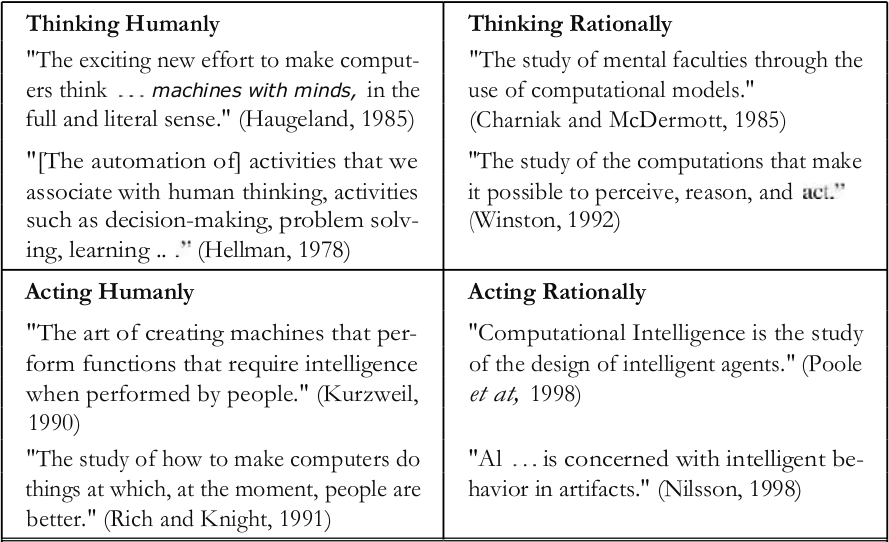
\includegraphics{different-povs-ai}
	\caption{Diferentes objetivos perseguidos por la~\glsentrylongsp{ai}. Las filas diferencian entre pensamiento o comportamiento mientras que las columnas separan entre inteligencia humana o el ideal de la inteligencia (racionalidad). Fuente: \textit{Artificial Intelligence: A Modern Approach ($3^{rd}$ Ed.)},~\cite{russell2003artificial}.}
	\label{fig:different-povs-ai}
\end{figure}

Volviendo al tema de la terminología, muchas de las diferentes técnicas se fueron agrupando dentro de diferentes áreas. Una de ellas es la conocida como \glsentrylong{ci}. Dado que persigue el mismo objetivo a largo plazo y que surje de la propia \ac{ai} parece lógico mantenerla como un subconjunto y no como un nuevo campo del conocimiento humano. Sin embargo, algunos autores abogan por que la \ac{ci} es un campo diferenciado de la \ac{ai}.

Podemos definir la \ac{ci} como la \enquote{\textit{rama de la \ac{ai} que aporta soluciones a \textbf{tareas específicas} de forma \textbf{inteligente} a partir del aprendizaje mediante el uso de \textbf{datos experimentales}}}. A diferencia de la aproximación clásica de la \ac{ai}, se buscan aproximaciones a las soluciones y no las soluciones exactas. Esto es debido a que muchos problemas son de naturaleza compleja, ya sea por la erlación entre sus multiplas variables, a la falta de información o a la imposibilidad de traducirlos a lenguaje binario.

Se puede fijar el año $1994$ como el que el término \ac{ci} nace como área, coincidiendo con el cambio de nombre del \textit{IEEE Neural Networks Council} a \textit{IEEE Computational Intelligence Society} (\url{http://cis.ieee.org/}). Poco antes, en $1993$, Bob Marks en su trabajo~\cite{bezdek1993intelligence} presentó las que él consideraba diferencias fundamentales entre la \ac{ai} y la \ac{ci} resumiéndolas en la siguiente frase.

\blockquote{Neural networks, genetic algorithms, fuzzy systems, evolutionary programming, and artificial life are the building blocks of CI.}

Durante estos años ganaba popularidad también el concepto del \ac{sc}. Éste engloba las técnicas que buscan resolver problemas con información incompleta o con ruido. Debido a que el conjunto de técnicas definidas como consituyentes del \ac{sc} son las mismas que las de la \ac{ci} algunos autores consideran ambos términos equivalentes. Nosotros consideramos que el \ac{sc} es un punto de vista de la computación más que de la \ac{ai} en contraposición con el \ac{hc}, y que la \ac{ci} hace uso de métodos del \ac{sc}\sidenote{El \ac{hc} es como se define la computación convencional frente al \ac{sc}. El \ac{hc} basa sus técnicas en aquellas basadas en modelos analíticos definidos de forma precisa y que en ocasiones requieren mucho tiempo de cómputo. Están basados en lógica binaria, análisis numérico, algoritmos y respuestas exactas. El \ac{sc} por otro lado es tolerante a la imprecisión y al ruido y tiende a llegar a soluciones aproximadas de manera más rápida. Se basa en modelos aproximados, emergencia de algoritmos y modelos estocásticos.}.

\section{Aprendizaje}

La resolución clásica a un problema suele ser la aplicación de una secuencia de instrucciones basadas en un conjunto de símbolos (e.g. una función escrita en el lenguaje de programación C). Esta forma de solucionar un problema no \textit{aprende} a solucionarlo. Se puede interpretar como que la solución está grabada en su memoria.

En la aproximación de la \ac{ci}, existen modelos y existen técnicas para hacer aprender esos modelos. La aplicación de dichas técnicas es lo que se conoce como \textbf{aprendizaje}. Las técnicas de aprendizaje en \ac{ci} se suelen clasificar en $2$ paradigmas:

\begin{itemize}
	\item \textbf{Supervisado}. El entorno presentado al modelo consiste en un conjunto de la forma $D = {(I_i, O_i) | \forall i \in \mathbb{N}}$, donde cada $O_i$ es la salida esperada del modelo a la entrada $I_i$. Los algoritmos tratarán de ajustar el modelo todo lo posible para que las salidas obtenidas sean lo más parecidas a las salidas originales. Este paradigma de entrenamiento suele estar relacionado con problemas de \textit{regresión}.
	\item \textbf{No supervisado}. Al modelo se le ofrece un conjunto de la forma $D = {I_i | \forall i \in \mathbb{N}}$, donde cada $I_i$ es una entrada al problema, pero del que no conocemos la salida. Los algoritmos dentro de esta categoría harán uso de estos datos para ir reajustando el modelo tratando de encontrar las estructuras ocultas entre dichos datos (e.g. patrones, correlaciones o clases). Es un paradigma de entrenamiento íntimamente relacionado con problemas de \textit{clasificación}.
\end{itemize}

Algunos autores hacen uso de técnicas pertenecientes a ambos paradigmas en forma de aproximación híbrida para suplir deficiencias u optimizar/acelerar el aprendizaje. Un claro ejemplo lo podemos ver en \cite{Hinton2006}, donde los autores hacen uso de \textit{autoencoders} como técnica no supervisada para la inicialización de los pesos de una red neuronal y posteriormente realizan un entrenamiento supervisado para la optimización es éstos.

Otros, añaden un paradigma más a estos dos existentes, el denominado aprendizaje \textbf{por refuerzo}. Sin embargo, nosotros preferimos considerarlo como un tipo de aprendizaje supervisado, ya que la única característica que lo diferencia es que es un tipo de aprendizaje que se usa en entornos de aprendizaje \textit{on line} ajustando el modelo en función de los estímulos percibidos del entorno por sus acciones sobre el mismo, y no en un entorno aislado previo de entrenamiento (\textit{off line}), como la práctica totalidad de técnicas supervisadas y no supervisadas.

\section{Técnicas en la \Glsentrylongsp{ci}}

Bajo el paraguas de la \ac{ci} se incluyen muchas técnicas diferentes, entre las cuales están las usadas en esta tesis. El resto de la sección describe el funcionamiento de cada una de estas técnicas.

\subsection{\Glsentrylongplsp{ann}}

Una \acrlongsp{ann} puede considerarse como una herramienta que trata de replicar las funciones cerebrales de un ser vivo de una manera muy fundamental (esto es, desde sus componentes más básicos, las neuronas) basándose para ello en estudios de neurobiología y de ciencia cognitiva moderna del cerebro humano\sidenote{Aún apoyándose en la topología y funcionamiento del cerebro humano para realizar el símil, lo cierto es que dichos modelos distan aún de considerarse \textit{cerebros artificiales}. La red neuronal más compleja hasta la fecha es la propuesta en~\cite{TraskANDREWTRASK}, con alrededor de $160.000$ parámetros a ser ajustados (podemos abstraernos y pensar en ellos como conexiones entre neuronas). Como dato anecdótico, se estima que sólo en el neocórtex (ver figura~\ref{fig:neocortex}) del ser humano existen alrededor de $20.000$ millones de neuronas, cada una de las cuales conectada a entre $100$ y $100.000$ neuronas vecinas (\cite{Pakkenberg1997}). Esto supone entre $2 \cdot 10^{12}$ y $2 \cdot 10^{15}$ conexiones. Tecnológicamente hablando, la sensación esque estamos aún a años luz de aproximarnos siquiera a la complejiadd de un cerebro humano.}.

\begin{figure}
	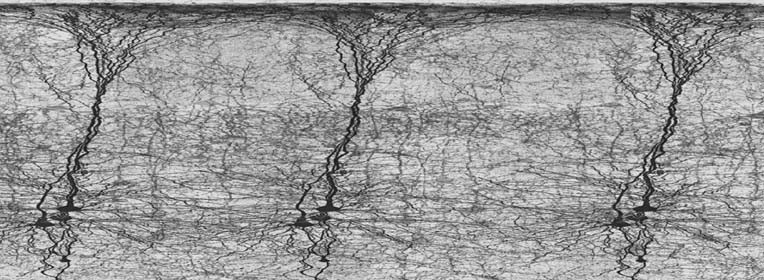
\includegraphics{neocortex}
	\caption{Una sección del neocórtex humano, región asociada a las capacidades cognitivas y que supone alrededor de un $76\%$ del volumen total del cerebro humano. Está distribuído en $6$ capas y miles de columnas que las atraviesan, cada una con alrededor de $10.000$ neuronas y un diámetro de $0.5mm$. Fuente: \textit{Blue Brain Project EPFL}, \url{http://bluebrain.epfl.ch/}.}
	\label{fig:neocortex}
\end{figure}

Una \ac{ann} es independiente del modelo del problema a solucionar. Se la puede considerar como una caja negra que aprende las relaciones que subyacen en los datos del problema para abstraer el modelo a partir de éstas. Estas características de aprendizaje y abstracción son los factores determinantes por los que son usadas en prácticamente todas las áreas de la ciencia y de la ingeniería (\cite{Du2006}).

\newthought{El modelo de neurona artificial} de McCulloch-Pitts introducido en el trabajo \enquote{A logical calculus of the ideas immanent in nervous activity} (\cite{McCulloch1943}, ilustración en la figura~\ref{fig:mccullocs-pitts-neuron-model}) es el considerado primer trabajo en la disciplina de las \acp{ann}, y aunque existen muchas y muy diferentes tipologías y formas de operar con redes, todas funcionan de la misma manera: unidades (i.e. neuronas) interconectados mediante enlaces por los que fluye la información de manera unidireccional, donde algunas de dichas unidades sirven de entrada al sistema (i.e. entradas o sensores), otras sirven de salida del sistema (i.e. salidas y actuadores) y otras como elementos internos (i.e. ocultas), y donde las conexiones se ajustan mediante un proceso denominado \textit{entrenamiento}.

\begin{figure}
	\missingfigure[figheight=4.6cm]{Figura del modelo artificial de McCullocs-Pitts}
	\caption{Variación de la representación del modelo de neurona artificial propuesto por McCullocs y Pitts. En éste, cada una de las entradas $x_i$ es incrementada o inhibida aplicando el producto con su peso asociado $w_i$. La activación vendrá determinada por la aplicación de una función (denominada \enquote{de activación}) a la suma de los valores. Esta variación en concreto incluye una entrada $x_0$ y un peso $w_0$ como bias de la neurona para la variación dinámica del umbral de activación.}
	\label{fig:mccullocs-pitts-neuron-model}
\end{figure}

Este primer modelo de neurona proponía una función escalón para determinar si la neurona se activaba o no (analogía al funcoinamiento de la neurona artificial). Posteriormente aparecieron nuevos modelos de neuronas diferentes funciones de activación. De éstas, las más comunes son las de tipo sigmoide\sidenote{
	Concretamente la función logística de pendiente $1$ definida como:
	\begin{equation}
		\frac{1}{1 + e^{-x}}
	\end{equation}
}.

\todo{Parrafito sobre la limitación de la neurona singular para dar hilo a las topologías}

\newthought{Existen diferentes topologías de redes neuronales} o arquitecturas dependiendo de qué forma toma el grafo que modela las neuronas y sus conexiones. En este caso, las redes neuronales pueden ser de dos tipos:

\begin{itemize}
	\item \textbf{Feed-Forward}. Sus grafos no contienen ninguń ciclo (figura XXX). Es la topología más usada en aplicaciones prácticas debido a su sencillez y su efectividad. En ellas el flujo de información sigue un camino desde las entradas hasta las salidas, sin ninguna retroalimentación. No es requisito que las neuronas se agrupen en capas, aunque suele ser la estructura común. A las redes de más de dos capas ocultas (i.e. las capas que se encuentran entre la capa de neuronas de entrada y la capa de neuronas de salida) se las denomina \enquote{profundas} o \textit{deep}. Algunos tipos pertenecientes a esta categoría pueden ser el Perceptrón [Rosemblat, 1957], el Perceptrón multicapa [Rumelhart et al., 1986], el algoritmo LVQ y su sucesor los Mapas Auto-Organizados [Kohonen, 1998].
	\item \textbf{Recurrentes}. Sus grafos contienen uno o más ciclos, de tal manera que el flujo de información de salida de una neurona puede llegar a afectar a su propio estado. Estas topologías representan de una forma más fiel las bases biológicas de las \ac{ann}, pero son más complejas a la hora de operar y entrenar. Algunos casos particulares de este tipo de arquitectura son las Redes de Hopfield [Hopfield, 1982] o las memorias LSTM (del inglés Long-Short Term Memory) [Hochreiter \& Schmidhuber, 1997].
\end{itemize}

\subsection{Aprendizaje en \glsentrylongplsp{ann}}

\section{\Glsentrylongsp{fl}}

La lógica matemática (y por extensión la teoría de conjuntos)\sidenote{Se puede establecer el siglo IV a.C. como el momento del nacimiento de la lógica dentro de la física Aristotélica, que permaneció inalterada hasta los trabajos de Galileo (cita?) y Newton (cita, seguramente el Principia Matematica) en el siglo XVI. d.C., momento en que se separó y permaneció como disciplina paralela perteneciente más al campo de la filosofía que de la física y la matemática. Empezó a relacionarse de nuevo con la matemática a principios del siglo XIX y a principios del siglo XX la lógica y la teoría de conjuntos pasaron a convertirse en partes indispensables la una de la otra. Por ello suelen ir de la mano cada vez que se habla de la una y de la otra. La evolución de la teoría de conjuntos (Cantor, finales del siglo XIX, buscar referencia) y su unión con la lógica es una época bastante convulsa dentro de la historia de la matemática pero esta tesis no es lugar para su desarrollo. Por ello se ofrece la referencia al libro \textit{La historia de la matemática} de Miguel de Guzmán (referencia. Poner la página. Lo mismo no es de aquí y es del libro de "Los lógicos", pero estoy casi seguro de que es aquí.) en caso de que el lector tenga interés en el tema.} tiene como misión servir de fundamento del razonamiento matemático. Se basa en la definición precisa y con rigor de un razonamiento evitando cualquier tipo de ambigiüedad y de contradicción. Es por ello que la lógica tradicional no suele servir como fundamento de razonamientos del mundo real.

Los conceptos que se manejan en el mundo real suelen ser vagos, llenos de imprecisiones. Además tienden a ser nombrados cualitativamente, no quantitativamente, y cuando existe una correspondencia, ésta suele estar marcada por la subjetividad de los términos.

Explicar lógica difusa y control difuso. Indicar los controladores difusos de segundo, tercer y sucesivos niveles.

\subsection{Teoría de conjuntos difusos}

A diferencia de los conjuntos tradicionales, los conjuntos difusos expresan el grado de pertenencia de un elemento a la categoría representada por el conjunto. La definición podría escribirse de la siguiente manera:

\TODO{Creo que habría que definir antes qué es un dominio}

\begin{definition}
	Sea $X$ una colección de elementos. Se define al \textbf{conjunto difuso} $F$ como un conjunto ordenado de pares de la forma $F = {(x, \mu_F(x)) | x \in X}$, siendo $\mu_F(x) \in [0, 1] \forall x \in X$.
	\label{def:fuzzy-set}
\end{definition}

La función de la definición~\ref{def:fuzzy-set} se denomina \textbf{función de pertenencia}, y caracteriza unívocamente a un conjunto difuso del dominio de $X$.

\TODO{Quizá aquí habría que decir qué es una partición de nu dominio}

\subsection{Operaciones entre conjuntos}

La unión, intersección y el complemento son operaciones básicas en la teoría de conjuntos. \TODO hablar aquí de tnorm, tconorm y complemento, pero someramente. No hay que enrollarse demasiado.

\subsection{Razonamiento}

En \cite{Ma} hay un capítulo de razonamiento que parece que está guay. Revisarlo un poco a fondo a ver si merece la pena tirar or ahí.

\subsection{Sistemas de inferencia difusa}

Los \acp{fis} o \acp{fcs} son sistemas que utilizan el razonamiento difuso para inferir una respuesta a partir de un conjunto de entradas. Habitualmente son divididos en tres bloques conceptuales, los cuales se ilustran en la figura XXX:

\begin{itemize}
	\item \textbf{Fuzzificación}. Traducir los valores de entrada en crudo del dominio sobre el que está definida cada variable lingüística a sus respectivos grados de pertenencia a conjuntos difusos a través de sus funciones de pertenencia. \TODO Ojo, algnuos controladores toman como valores de entrada conjuntos difusos según \cite{Ma}. Habrá que buscar sobre ello.
	\item \textbf{Inferencia}. Realiza todo el proceso de razonamiento difuso a partir del conjunto de reglas qeu dan significado a este controlador difuso.
	\item \textbf{Defuzzificación}. Traduce los conjunto difuso resultado del proceso de inferencia a valores del los dominios sobre los que están definidos dichos conjuntos difusos. \TODO En un sugeno, la salida es una función directamente así que se podría especificar que en un tipo Sugeno,se puede ver como que la salida son sólo singletones, manteniendo la generalización del proceso de funcionamiento de un \ac{fis}.
\end{itemize}

Hablar someramente de los tres tipos clásicos que se usan, e indicar que al final los más usados son el Mandamni y el Sugeno. Añadir también quizá una tabla comparativa enter los tres o al menos entre los dos principales:

El consecuente de un \ac{fis} de tipo Mandamni siempre es un conjunto difuso. Por tanto, el proceso de sacar un valor crisp es costoso. Lo bueno, se mantiene significado semántico de las salidas. El consecuente en un Sugeno es un valor, y se puede decir que no necesita proceso de defuzzificación. Si embargo, la respuesta pierde significado semántico si la suma de la fuerza de salida no es 1 (no entiendo qué quiero decir con esto).

\section{\Glsentrylongsp{cev}}

Otra de las técnicas inspiradas\sidenote{Destacar que los algoritmos están \textit{inspirados} y no \textit{basados en}. Los algoritmos no son réplicas con pequeñas modificaciones, sino que toman forma a partir de ideas que surgen de observar los comportamientos existentes.\TODO{Ojo que en redes neuronales también hablo de \enquote{inspirados}. A lo mejor tengo que hacer esta aclaración antes y quitarla de aquí.}} en principios biológicos es la de la \gls{cev}. Esta área de la \gls{ci} trabaja sobre algoritmos iterativos inspirados en la síntesis evolutiva moderna o \textit{neodarwinismo}\sidenote{\TODO{Explicar diferencia entre darwinismo y neodarwinismo}.}.

Existe un conjunto de algoritmos denominados \gls{si} que también son algoritmos iterativos estocásticos inspirados en cómo se comportan sistemas colectivos donde el conocimiento emerge de la interacción de individuos, ya se trate de sistemas naturales como por ejemplo el de las bandadas de murciélagos (\cite{Yang2010}) o de sistemas artificiales como sistemas de partículas abstractas (\cite{Artyukhin2014}). Algunos autores consideran este conjunto de algoritmos como pertenecientes al subcampo de la \gls{cev}, pero nosotros consideramos a la \gls{si} como un subcampo independiente dado que el adjetivo \textit{evolutivo} no es característico de este tipo de algoritmos\sidenote{El punto de vista de los autores que lo incluyen es que la evolución no sólo ha sido la razón de la adaptación de los individuos, sino que también es la causante de comportamientos inteligentes grupales. Y, aunque es una apreciación cierta, el adjetivo \textit{evolutivo} se refiere a cómo trabajan los algoritmos, no a lo que ha propiciado la evolución en la naturaleza.}.

\subsection{\glsentrylongplsp{ga} y sus variantes}

Desde nuestro punto de vista, podemos decir que la \gls{cev} es el área que trabaja con \gls{ga} y, aunque la afirmación puede resultar reduccionista, veremos como no es tal.

Un \gls{ga} es un algoritmo iterativo estocástico donde se aplica una serie de pasos inspirados en el funcionamiento de los mecanismos de la evolución y la genética a una población de individuos donde cada uno simboliza una solución a nuestro problema. Éstos fueron introducidos por John Henry Holland en su libro \textit{\enquote{Adaptation in Natural and Artificial Systems}} (\cite{Holland1975} \TODO{a mí me suena que fueron introducidos a principio de los años 60, y he encontrado autores que dicen eso, pero no encuentro ninguna referencia anterior a ésta de 1975}) y constituyen una familia de soluciones con mucho éxito en problemas de aprendizaje, búsqueda y optimización.

\begin{figure}
	\missingfigure[figheight=3.5cm]{Esquema general de funcionamiento de un algoritmo genético}
	\caption{Esquema general del funcionamiento de un \glsentrylong{ga}. Se parte de una población de individuos y en iteraciones de selección-recombinación-mutación-reemplazo se va mejorando la población hasta llegar a una solución que, si bien no tiene por qué ser necesariamente la mejor, es lo suficientemente buena como para ser válida.}
	\label{fig:genetic-algorithm-schema}
\end{figure}

La figura~\ref{fig:genetic-algorithm-schema} muestra un esquema genérico del funcionamiento de un algoritmo genético. Los principales pasos dentro del algoritmos son los siguientes:

\begin{itemize}
	\item \textbf{Inicialización}. El algoritmo crea una \textit{población} de individuos donde cada uno representa una posible aproximación a la solución del problema a resolver.
	\item \textbf{Selección}. Al igual que en la naturaleza, donde el individuo más apto tiene la mayor probabilidad de sobrevivir y tener descendencia con sus características diferenciadoras, en un \gls{ga} el individuo más apto (que represente una solucion más cercana a la buscada) es el que más probabilidades tiene de ser seleccionado para transmitir sus características a las sucesivas poblaciones.
	\item \textbf{Recombinación}. Tras seleccionar a uno o más individuos, existe una probabilidad (generalmente alta) de que éstos generen uno o más individuos con una composición genética resultado de la combinación de éstos. El algoritmo general habla de selección de $2$ individuos y del operador \enquote{cruce}, pero es posible generalizarlo para que el cruce vaya de $1$ individuo (i.e. no hay cruce, es traspaso de una versión de los genes) a $n$ (i.e. todos los individuos tienen probabilidad de transmitir su genotipo, ya sea directamente o aplicando una función a combinaciones de éstos). La recombinación consigue que la composición genética de los individuos (que probablemente sea buena porque han sido seleccionados frente al resto de individuos) se perpetúe en sucesivas poblaciones.
	\item \textbf{Mutación}. Una vez generada una descendencia en la recombinación (o no, pueden ser los individuos originales), los individuos tiene cierta probabilidad (por lo general baja) de que su genotipo sea modificado aleatoriamente. Esto puede hacer del individuo resultante una mala solución, pero también puede hacer que la solución sea nueva o si no, al menos ofrecer más variedad genética a la población.
	\item \textbf{Reemplazo}. Tras uno o más pasos de selección, recombinación y mutación, los nuevos individuos generados reemplazarán a individuos de la población inicial. En general la población en un \gls{ga} contiene el mismo número de individuos según pasan las generaciones, pero no es un requisito fundamental.
\end{itemize}

Sin embargo, dentro de la \gls{cev} siguen existiendo familias de algoritmos consideradas, en un principio, diferentes:

\begin{itemize}
	\item \textbf{\glspl{es}}. Esta familia de algoritmos nacen casi a la par con los \gls{ga} por parte de Ingo Rechenberg (\cite{Rechenberg1973}). Se caracterizan principalmente por ser algoritmos iterativos inspirados en la evolución pero que basan su funcionamiento en los pasos de selección y mutación y donde el reemplazo es total. Es evidente que se pueden considerar como una especialización de algoritmo genético donde la recombinación y el reemplazo parcial pasan a un segundo plano.
	\item \textbf{\gls{gp}}. Es en realidad una aplicación de \gls{ga} a la generación de programas. Sus comienzos se pueden trazar hasta Koza13, quien representa los genotipos de los individuos como árboles sintácticos en lugar de cadenas de símbolos (la representación de un genotipo clásico). Aunque algunos autores lo consideran una familia de algoritmos independientes, en realidad son algoritmos genéticos con diferente representación de individuos y, por tanto, diferentes operadores de recombinación y de mutación.
\end{itemize}

\subsection{El balance entre biodiversidad y presión selectiva}

El buen funcionamiento de un \gls{ga} depende del equilibrio de dos conceptos inversamente relacionados: la biodiversidad y la presión selectiva.

\newthought{La biodiversidad} se refiere a la riqueza genética que existe entre los individuos de nuestra población. Los individuos mejor adaptados poseen rasgos característicos resultado de combinaciones de uno o más genes en sus genotipos\sidenote{}.Cuando la variedad genética de una población de individuos es baja, la tendencia es que los individuos resultantes de la recombinación tiendan a perpetuar esos pocos rasgos característicos y por tanto se depende de las mutaciones para la aparición de ragos genéticos únicos que mejoren las soluciones. Aumentando la diversidad genética se favorece la aparición de nuevos 
Aquí hablamos un poquito de qué es la biodiversidad, qué es la presión selectiva y por qué es importante mantener ambos.

\newthought{La presión selectiva}, por otro lado
Alguna gráfica molona con algún ejemplo que haga con pynetics y reafirmar de cómo funciona este balance.

Luego, hablar sobre el fitness como medida de calidad de una solución. Hablar de representación de cuanto más alto mejor, cuanto más bajo mejor y representación de 0 a 1 en función del error. Se puede a lo mejor hablar también de lo que he visto hoy de SVM de gaussian kernel para calcular el error.

\subsection{Representación de individuos}

Hablar de la relación entre espacio de individuos, espacio de soluciones y su puta madre.

Hablar de representación de lista de símbolos finitos, de símbolos infinitos, representación en árbol y en árbol generado a partir de árbol gramatical.

\subsection{Manipulación de individuos: recombinación y mutación}

Recombinaciones clásicas para los individuos de antes. Matizar que la recombinación puede depender mucho del problema.

Recombinaciones con árboles y sus problemas principales.

\subsection{Reemplazo de individuos}

Tasa generacional, diferencia entre generacional vs. steady-state y variación de elitismo es en realidad una tasa generacional donde deja un individuo.

Algoritmos de reemplazo clásicos.

\subsection{Variaciones y operadores adicionales}

Hablar de los catastróficos y los que me falten. Hay que encontrar más, porque me parece ridículo un apartado para sólo uno.

\subsection{\glsentrylongpl{ga} distribuidos}

\subsection{Optimización de \glsentrylongpl{fis} mediante \glsentrylongpl{ga}}

\section{Agentes inteligentes}
\label{ch:ci:s:agent-concept}

Si echamos un poco la vista atrás, en la figura~\ref{fig:different-povs-ai} se mostraban los cuatro objetivos perseguidos por la \ac{ai}. En uno de ellos en particular se la entiende como el estudio del conseguir que las entidades (e.g. sistemas, software, \ldots) actúen de la manera más inteligente posible. A dichas entidades se las conoce como \textit{agentes}, concretamente en este contexto como \textit{agentes inteligentes}\sidenote{En realidad los autores prefieren denominarlo \textit{agente racional}, dado que captura la esencia de lo que es un comportamiento inteligente. Sin embargo, según esta definición, hasta un elemento tan rudimentario como un termostato puede ser considerado como elemento inteligente, ya que realiza siempre la mejor acción para cumplir sus objetivos, por simples que puedan parecer. Dónde está el límite entre qué es y que no es un agente inteligente cae dentro de los dominios de la filosofía.}. Sin embargo, si es difícil encontrar un consenso en la definición de agente más lo es a la hora de definir cuándo la conducta de éstos es inteligente.

Lo que sí existe es una serie de características comunes que se repiten a lo largo de la literatura (figura~\ref{fig:agent-properties}):

\begin{itemize}
	\item Operan siempre en un \textbf{entorno}, ya sea éste físico (e.g. una red de carreteras para un vehículo autónomo) o virtual (e.g. un cliente de correo electrónico para un clasificador de spam).
	\item Tienen la capacidad de \textbf{percibir} el entorno por medio de \textit{sensores} y de \textbf{actuar} sobre él por medio de \textit{actuadores}.
	\item Son \textbf{autónomos} en el sentido de que pueden actuar sin intervención externa (e.g. humana u otros agentes) teniendo control sobre su estado interno y su comportamiento. Algunos autores les presuponen una autonomía absoluta mientras que otros hablan de que sólo es necesaria cierta autonomía parcial.
	\item Tienen \textbf{objetivos} a cumplir, actuando para ello sobre el entorno de la manera que les indique su comportamiento.
	\item Pueden ser \textbf{sociales}, es decir, tienen la capacidad de comunicarse con otras entidades (e.g. otros agentes) para llevar a cabo sus objetivos.
\end{itemize}

Por tanto nosotros usaremos la siguiente definición: Un agente es una entidad física o virtual que realiza una acción\sidenote{En \cite{russell2003artificial} se define como \textit{\enquote{\ldots just something that acts}} alegando que la palabra \textit{agent} proviene del latín \textit{agere}. Para clarificar esto, \textit{agere} es la forma verbal para \textit{hacer}, pero imprime un significado de movimiento/actividad diferente que no tiene mucho que ver con \textit{hacer} como forma verbal para \textit{crear} o \textit{dar forma} (de lo que se ocupa el verbo \textit{facere}). Por ello, el verbo \textit{actuar} es un verbo que se relaciona con \textit{agere} y de ahí la definición.} de manera total o parcialmente autónoma dada una secuencia de percepciones del entorno en el que se ubica.

\begin{figure}
	\missingfigure[figheight=3.5cm]{Modelo genérico de agente con sus características típicas}
	\caption{Esquema de un agente y sus propiedades. Aunque no existe una definición comúnmente aceptada de agente, sí que existe una serie de propiedades que los que los identifican. Es autónomo, opera realiza acciones sobre un entorno dependiendo de las percepciones que le llegan de éste y tiene la capacidad de comunicarse con el resto de elementos, incluídos otros agentes.}
	\label{fig:agent-properties}
\end{figure}

Pero, ¿qué hace a un agente inteligente? Según algunos autores, el hecho de que posea unos objetivos y autonomía suficiente para cumplirlos ya denota inteligencia (\TODO{encontrar el trabajo y citar}). Según otros, es necesario que el comportamiento sea flexible, esto es, que sea reactivo (reacciona ante el entorno que percibe), proactivo (iniciativa para tratar de cumplir sus objetivos) y social (capaz de interactuar con otros agentes para cumplir sus objetivos) \cite{Wooldridge1995}. Y otros directamente exigen, además, un comportamiento racional a la hora de cumplir los objetivos para calificarlo de inteligente (\TODO{encontrar el trabajo y citar}).

Por tanto, asumiremos la definición ofrecida por \cite{russell2003artificial} donde, se indica que un agente es considerado \textbf{agente inteligente} cuando éste realiza la mejor acción posible (según un criterio de medida). En este contexto, \enquote{la mejor acción posible} se refiere en términos de objetivos y comprensión del entorno, que puede ser o no correcta\sidenote{Que la comprensión del entorno no sea totales un factor clave que diferencia la racionalidad de la omnisciencia. La omnisciencia significa conocer el resultado de toda acción antes de realizarla y por tanto implica el conocimiento de absolutamente todos los detalles del entorno.La racionalidad existe dentro de un contexto de conocimiento limitado.}.

Las nociones de agentes inteligentes y la de \ac{ci} van de la mano. Esto es debido a que su definición funciona a la perfección para las técnicas de la \ac{ci}, esto es, agentes autónomos que perciben el entorno (problema) y actuan de la mejor manera posible sobre él (resuelven) de acuerdo a su conocimento del medio y su estado interno (en base a algoritmos como \ac{ann}, \ac{fl}, \ldots). Por ello desde mediados de los años 1990 el concepto de agente inteligente ha ganado tanta popularidad\sidenote{Tanto es así que en algunos trabajos se define el objetivo de la \ac{ai} como la implementación de la función agente, esto es, la función que realiza la correspondiencia de una percepción a una acción, para un problema dado.}.

\subsection{Tipos de entorno}

La tupla \textit{(entorno, agente)} es esencialmente una metáfora para referirse a la tupla \textit{(problema, solución)} por lo que existen casi tantos entornos diferentes como problemas.

Afortunadamente es posible caracterizar los entornos de acuerdo a un conjunto de propiedades o dimensiones. Este conjunto es usado por la totalidad de la literatura a la hora de caracterizar entornos:

\begin{itemize}
	\item \textbf{Observable}. Un entorno es \textbf{totalmente observable} cuando el agente es capaz de captar toda la información relevante para la toma de una decisión y no necesita mantener ningún modelo interno del entorno, \textbf{parcialmente observable} cuando la información obtenida es incompleta o tiene ruido y \textbf{no observable} cuando el gente no posee sensores.
	\item \textbf{Multiagente o. monoagente}. Un entorno es \textbf{multiagente} cuando requiere de múltiples agentes interactuando para llegar a una solución mientras que es \textbf{monoagente} cuando sólo requiere de uno para ello.
	\item \textbf{Determinista o. no determinista}. Si el estado del entorno actual depende totalmente del estado anterior, se dice que el entorno es \textbf{determinista}. Si no es así, se considera \textbf{no determinista} o \textbf{estocástico}\sidenote{En general, los entornos del mundo real tienden a ser tan complejos que es imposible para un agente abarcar todos los aspectos medibles de éste. Por lo tanto, sea o no la naturaleza del entorno determinista, en general se suele suponer éste como no determinista.}.
	\item \textbf{Episódico o. secuencial}. Un entorno en el que las acciones se dividen atómicamente donde cada una de ellas conlleva un ciclo de (percepción, decisión, acción) y sin relación una con otra se denomina episódico. Si en lugar de ello la acción del agente puede afectar a las decisiones futuras se dice que el entorno es \textbf{no episódico} o \textbf{secuencial}.
	\item \textbf{Estático o. dinámico}. Si durante la toma de decisioń en entorno no cambia, se dice que el entorno es \textbf{estático}. En caso contrario, se dice que es \textbf{dinámico}.
	\item \textbf{Discreto o. continuo}. Esta dimensión en realidad se divide en cuatro, estado del entorno, tiempo en el entorno, percepciones y acciones. La dimensión es \textbf{discreta} cuando ésta se divide en una partición discretizada, y \textbf{continua} cuando no. Por ejemplo, en el Juego de la Vida de Conway, si se modela en un sistema multiagente, tanto el estado (i.e. tablero) como el tiempo (i.e. turnos) como las percepciones y acciones están discretizadas. Sin embargo, en un entorno de conducción automática se puede determinar que las cuatro dimensiones son continuas.
	\item \textbf{Conocido o. desconocido}. Un entorno es \textbf{conocido} cuando es posible determinar cuál va a ser el resultado de una acción. Si por el contrario no es posible, entonces se dice que es \textbf{desconocido}.
\end{itemize}

\section{Arquitecturas}

Existe una serie de arquitecturas básicas o tipos de agentes que dependen principalmente de cómo perciben el entorno y de qué forma se comportan aunque, dependiendo de los autores, las nomenclaturas, tipologías y esquemas pueden variar. Por ello, hemos decidido ofrecer una abstracción donde poner de manifiesto las partes comunes y no comunes entre arquitecturas.

\begin{figure}
	\missingfigure[figheight=3.5cm]{Arquitectura básica de un agente}
	\caption{Arquitectura básica de un agente. Aunque existen múltiples arquitecturas diferentes, todas se basan en la misma estructura. El agente percibe el entorno, lo interpreta y toma la decisión de cómo actuar sobre él.}
	\label{fig:agent-basic-architecture}
\end{figure}

La figura~\ref{fig:agent-basic-architecture} muestra el esquema de las partes principales de un agente. En general, todo arquitectura de agente inteligente está cortada por el mismo patrón y obedece al siguiente funcionamiento:

\begin{enumerate}
	\item El agente, a través de sus \textbf{sensores}, percibe el entorno en el que éste se mueve.
	\item De acuerdo a cómo recordamos el entorno (llamémoslo \textbf{modelo del entorno}), el agente genera una \textbf{interpretación del entorno} tal y como supone el agente que es. Esto es, percibe el entorno y, de acuerdo a sus sensaciones, lo entiende de una determinada forma.
	\item Esta interpretación del entorno es pasada a un proceso de \textbf{inferencia} el cual, en función la implementación para la consecución de sus objetivos, generará una serie de acciones a realizar sobre el entorno.
	\item Estas acciones serán ejecutadas sobre el entorno a través de una serie de \textbf{actuadores}, provocando probablemente una modificación en éste que será percibida de nuevo en momentos sucesivos.
\end{enumerate}

La primera diferencia clave surge en la manera que se ofrece al bloque de inferencia la interpretación del entorno y genera la primera clasificación (figura~\ref{fig:memory-vs-amnesia-in-agents}):

\begin{figure}
	\missingfigure[figheight=3.5cm]{Arquitectura básica de un agente}
	\caption{Ilustración de la diferencia entre un agente sin modelo de entorno y uno con modelo de entorno. Cada acción realizada por el agente con modelo de entorno tiene en cuenta el estado del entorno en momentos pasados. El agente sin modelo de entorno actúa tal y como interpreta el entorno en cada momento, como si sufriese de amnesia.}
	\label{fig:memory-vs-amnesia-in-agents}
\end{figure}

\begin{itemize}
	\item \textbf{Sin modelo de entorno}. Si el agente ofrece su interpretación del entorno directamente, sin hacer uso de información histórica sobre el entorno que se ha movido. Otras formas de denominar a estos agentes es como \textit{agentes reactivos} o \textit{simple-reflex agents} (\cite{russell2003artificial}). Sin embargo, los términos \textit{reactivo} o \textit{reflex} para algunos autores se refieren a la forma de inducción de acciones a partir de percepciones, y por ello preferimos la denominación \textit{sin modelo de entorno}.
	\item \textbf{Con modelo de entorno}. El agente genera su interpretación más detallada del entorno a partir de las percepciones que llegan desde los sensores y de el histórico del entorno que mantiene. Otras formas de llamarlo es \textit{agentes con estado} o \textit{Model-based}, pero lo hemos denominado de esta manera para diferenciar que el modelo que se mantiene en este punto pertenece únicamente al entorno.
\end{itemize}

\begin{figure}
	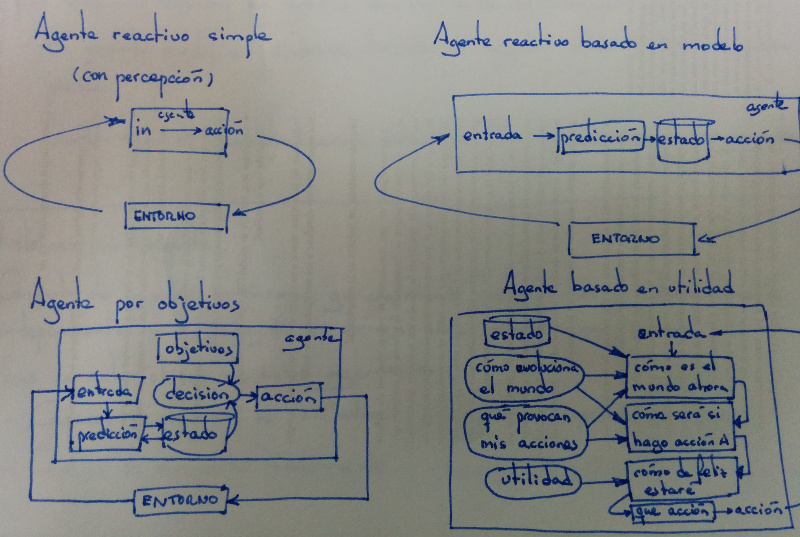
\includegraphics{agent-types}
	\caption{Distintas arquitecturas de agentes en función del comportamiento. Dependiendo de las acciones a realizar, se identifican tres tipos, los reactivos que aplican una acción sin proceso deductivo y los basados en modelo y utilidad (en algunos contextos denominados deliberativos) que basan su comportamiento en alguna forma de deducción.}
	\label{fig:agent-types}
\end{figure}

La siguiente clasificación viene motivada por la forma de deducir el conjunto de acciones a ser aplicadas por parte de los sensores. En este sentido podemos identificar tres tipos distintos de agentes (figura\ref{fig:agent-types}):

\begin{itemize}
	\item \textbf{Reactivos}. Son aquellos donde el uso de un proceso de razonamiento explícito es demasiado costoso para producir una conducta en un tiempo aceptable. Se suelen implementar como correspondencias (percepción $\rightarrow$ acción) sin ningún razonamiento adicional.
	\item \textbf{Basados en objetivos}. Plantean una deducción de forma que determinan cuál sería el estado del entorno tres aplicar varias o todas las acciones que puede realizar. En base a los resultados, selecciona la acción que se corresponde con sus propios objetivos.
	\item \textbf{Basados en utilidad}. Éstos plantean una deducción similar a los basados en objetivos con la diferencia de que, mientras los primeros sólo diferencian entre entorno objetivo o no objetivo, éstos asignan un valor (i.e. \textit{utilidad}) a cada uno de los escenarios de entorno posibles para seleccionar el mejor (e.g. el que mayor utilidad tiene).
\end{itemize}

En la literatura se describen muchos tipos de agente, como por ejemplo los agentes BDI (Believe-Desire-Intention) o los agentes lógicos (i.e. el entorno se representa con reglas lógicas y se infiere mediante métodos como por ejemplo deducción lógica o prueba de teoremas). Sin embargo, éstos pueden definirse en los términos aquí expuestos (figuras~\ref{fig:agent-basic-architecture}, \ref{fig:memory-vs-amnesia-in-agents} y \ref{fig:agent-types}). 

\subsection{\Glsentrylongsp{mas}}

Son aquellos sistemas compuestos de dos o más agentes que interactúan de alguna manera para llegar a una solución.

Cuando los agentes son inteligentes y el problema cae dentro del dominio de la \gls{ai}, el ámbito de estudio es el de la \gls{dai}, la rama dedicada a la resolución de problemas mediante procesamiento descentralizado.

Desde el punto de vista de la ingeniería de sistemas, y a pesar del aumento de complejidad, los \ac{mas}, al ser sistemas inherentemente descentralizados, ofrecen múltiples ventajas frente a los sistemas centralizados tradicionales:

\begin{itemize}
	\item Los sistemas son más robustos y fiables frente a fallos, ya que los agentes son autónomos e independientes del resto.
	\item La modificación del sistema se puede realizar sobre la marcha, agente a agente sin necesidad de parar el sistema al completo.
	\item Su diseño fuerza a desacoplar las dependencias entre agentes.
	\item Son inherentemente paralelizables y por tanto pueden llegar a ser más eficientes que sus homólogos centralizados. Este punto es quizá el más controvertido, ya que esta ganancia en eficiencia se puede perder rápidamente en función de la cantidad de comunicación existente entre agentes.
	\item Debido al nivel de complejidad alcanzado en los sistemas existentes en la actualidad, la computación se distribuye a través de múltiples sistemas, normalmente heterogéneos. La tendencia además es a la alza. La definición de los \ac{mas} hace natural su implementación en este tipo de arquitecturas.
\end{itemize}
	
Desde el punto de vista de la \gls{ai} podemos añadirles la ventaja de que permiten el estudio de conductas complejas de poblaciones a partir del comportamiento de sus elementos básicos, facilitando el estudio de modelosy de teorías sobre éstos.

\newthought{La comunicación entre agentes}, se trata de una característica clave en un \gls{mas}, ya que para denominarse de esta manera dos o más agentes deben interactuar (i.e. comunicarse) entre si. Esta interacción puede implementarse de diversas maneras\sidenote{Las formas clásicas de comunicación son el de paso de mensajes, los sistemas de pizarra y la estigmergia. Para los dos primeros existen dos propuestas para estándar de lenguaje de comunicación, \Ac{kqml} (\cite{Finin1994}) y \Ac{acl} (\cite{Poslad2007}). La tercera forma de comunicación suele ser muy dependiente del problema y no se apoya en lenguajes estándares. Se trata de una forma de comunicación basada en la modificación del entorno, como la efectuada por las hormigas en la búsqueda de alimento, donde éstas dejan rastros de feromonas modificando el entorno para modificar el comportamiento del resto de la colonia.} y siempre toman una o las dos formas siguientes (figura~\ref{fig:communication-between-agents-in-mass}):

\begin{itemize}
	\item \textbf{Cooperación}. Los agentes intercambian información entre sí para llegar a una solución. Esta solución puede ser fragmentada (i.e. cada agente posee parte de la solución y se comunican para ir avanzando de forma común hacia la solución global) o poseerla uno o varios agentes que hacen uso de más agentes para ir avanzando la solución.
	\item \textbf{Competición}. Los agentes compiten dentro de un entorno, generalmente mediante la adquisición de recursos limitados. Un ejemplo de este tipo de sistemas multiagente puede ser aquellos sistemas de vida artificial.
\end{itemize}

\begin{figure}
	\missingfigure[figheight=3.5cm]{Una ilustración de algún entorno de vida artificial donde los agentes compiten y uno de algo donde cooperen}
	\caption{Ilustración de la diferencia entre un agente sin modelo de entorno y uno con modelo de entorno. Cada acción realizada por el agente con modelo de entorno tiene en cuenta el estado del entorno en momentos pasados. El agente sin modelo de entorno actúa tal y como interpreta el entorno en cada momento, como si sufriese de amnesia.}
	\label{fig:communication-between-agents-in-mass}
\end{figure}

\TODO{Aquí una figura de un entorno de vida artificial y un entorno multiagente donde cooperen}

\chapter{Simulación de tráfico}
\label{ch:sota-traffic-simulation}

El tráfico es un sistema caótico en el que intervienen un número muy elevado de diferentes variables, muchas de las cuales relacionadas entre si. Debido a esto, obtener modelos exactos de tráfico es una tarea prácticamente imposible y es por ello que la mayoría del trabajo cuyo objetivo es la predicción se realice en base a simuladores.

Los simuladores de tráfico son herramientas de software que, usando diferentes modelos, describen el tráfico como sistema, permitiendo:

\begin{itemize}
	\item Extraer resultados y conclusiones de escenarios de tráfico determinados.
	\item Implementar técnicas de tráfico sin necesidad de alterar el tráfico real.
	\item Reproducir exactamente un escenario.
	\item Introducir modificaciones en puntos determinados (e.g. espaciales o temoprales) de un escenario conocido para evaluar la divergencia en su evolución.
\end{itemize}

Los objetivos en la simulación de tráfico son los de hacer que los modelos se parezcan lo máximo posible a la realidad. En este capítulo vamos a ver cuál es la realidad actual de este tipo de simuladores, cuáles son sus diferentes tipologías y maneras de modelar los diferentes aspectos del tráfico y, posteriormente, realizaremos una evaluación de cuáles son los idóneos para nuestro trabajo.

Limitaremos el estudio no obstante a los simuladores de vehículos, obviando otros tipos de simulación de tráfico que no tienen que ver con esta temática, como por ejemplo los orientados a la evaluación de sistemas de señalización inteligentes (e.g.~\cite{jin2016evaluation}) o a la estimación de emisiones (e.g.~\cite{quaassdorff2016microscale}).

\section{Clasificación de simuladores de tráfico}

Los aspectos simulables y medibles del problema tráfico son muy diversos, dependiendo sobre todo del nivel de complejidad del tráfico\sidenote{Modelar una vía por la que circula un centenar de coches no es lo mismo que modelar una ciudad donde circulan millones.}, de qué queremos medir\sidenote{Evaluar a un conductor en una situación determinada o evaluar la evolución del flujo de tráfico en un cuello de botella causado por un accidente.} y de cómo lo modelamos\sidenote{Un autómata celular se modela de forma diferente a un modelo lineal de vías o carriles.}.

El resto de la sección ofrece una visión de las diferentes categorías en las que se clasifican los simuladores de tráfico.

\subsection{Tipos de simulador en función de la complejidad}

La complejidad en una simulación se refiere al nivel de detalle al que queremos llegar a la hora de modelar nuestra solución. Es evidente que según aumentamos el detalle en la simulación aumenta la cantidad de cálculo. Por ejemplo, si queremos modelar el comportamiento de $10$ billones de canicas cayendo por un tubo es considerablemente más eficiente modelarlas como un fluido con una serie de propiedades características que como una colección de elementos individuales, cada uno con sus propiedades (e.g. masa, aceleración, ...) e interaccionando entre sí.

\begin{figure}
	\centering
	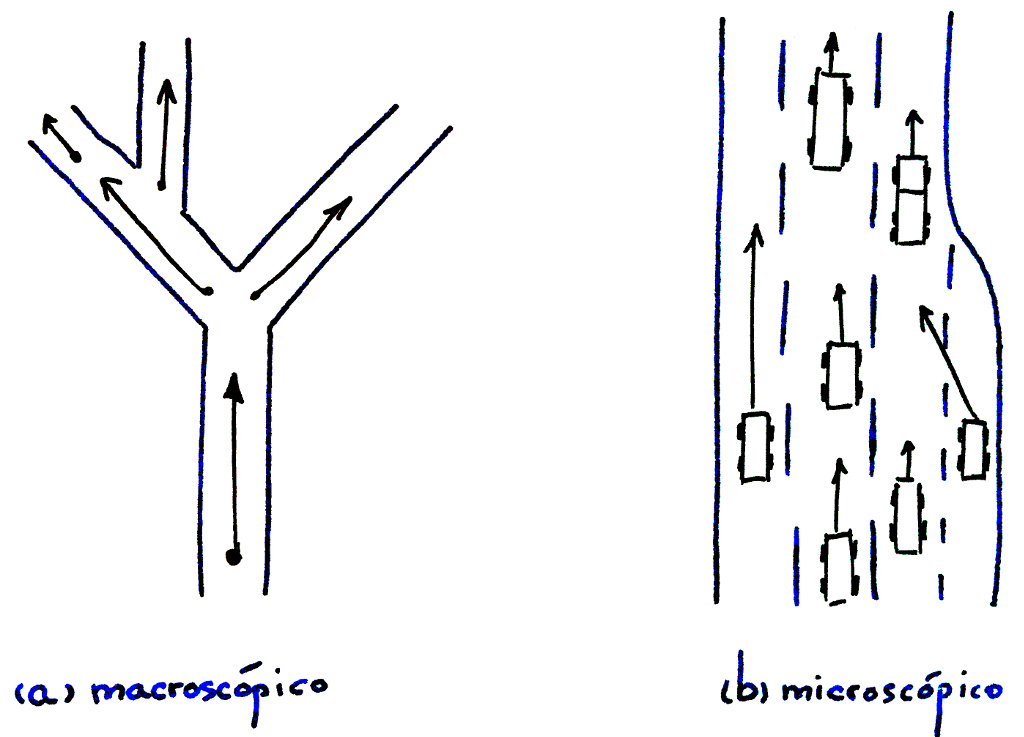
\includegraphics{images/granularities-in-traffic-simulation}
	\caption{Taxonomía clásica de los simuladores en función de la granularidad (complejidad) de la simulación.}
	\label{fig:granularities-in-traffic-simulation}
\end{figure}

En el caso de los simuladores de tráfico es lo mismo. En éstos existe un amplio intervalo de granularidades, desde por ejemplo el flujo de entrada en una autovía hasta el consumo de carburante de un vehículo en ciudad. Lo más común es clasificar los simuladores dentro de dos grandes grupos, los cuales se ilustran en la Figura~\ref{fig:granularities-in-traffic-simulation}:

\begin{itemize}
	\item \textbf{Microsimulación} o simulación de tipo \textbf{micro}. Su objetivo es estudiar, desde un punto de vista de granularidad fina como puede ser vehículos o peatones, las micropropiedades del flujo de tráfico como, por ejemplo, los cambios de carril, las aproximaciones a vehículos delanteros o los adelantamientos, para evaluar su comportamiento. Tiene dos principales ventajas, la posibilidad de estudiar el tráfico como un todo a partir de sus elementos más simples (ofreciendo una representación más fiel de éste) y la posibilidad de estudiar cada elemento por separado. Sin embargo, la principal desventaja de este tipo de modelos es que cada elemento de la simulación requiere de cómputo independiente y por tanto simulaciones con alto contenido de elementos pueden llegar a ser inviables\sidenote{Existen técnicas de computación distribuida que superan ampliamente los límites impuestos por la computación en un único nodo, por ejemplo, el simulador de IBM \textit{Megaffic}. Éste implementa un modelo de granularidad micro donde cada elemento es un agente independiente (i.e. sistema multiagente) usando para ello entornos con cientos de núcleos de proceso que proveen de capacidad suficiente para modelar ciudades enteras como Tokio (ver~\cite{Osogami2012} y~\cite{Suzumura2012}).}.
	\item \textbf{Macrosimulación} o simulación de tipo \textbf{macro}. Este tipo de modelos centran su esfuerzo en estudiar el flujo de tráfico como un todo, explorando sus macropropiedades (e.g. evolución del tráfico, efectos onda, velocidad media o flujo en vías). Su ventaja principal es que a nivel macroscópico permiten estudiar propiedades que a nivel microscópico requeriría una cantidad ingente de recursos. Sin embargo, con este modelo es imposible obtener información precisa de un elemento en particular del tráfico.
\end{itemize}

Aunque esta es la categorización típica de modelos, en la literatura aparecen otros tipos de modelo con granularidades que pueden considerarse no pertenecientes a ninguno de estos dos conjuntos. Este es el caso de los simuladores de tipos \textbf{sub-micro} y los \textbf{meso} (ver figura~\ref{fig:mesoscopic-and-submicroscopic-simulation}). 

\begin{figure}
	\centering
	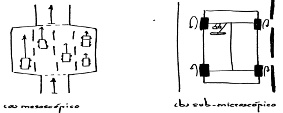
\includegraphics{images/mesoscopic-and-submicroscopic-simulation}
	\caption{Aproximaciones alternativas de modelos en función de la complejidad. Ejemplo de mesosimulación como ventana de microsimulación dentro de un flujo en un macrosimulador (e.g. \cite{munoz2001integrated}) y ejemplo de submicrosimulación donde se modelan componentes internos del vehículo.}
	\label{fig:mesoscopic-and-submicroscopic-simulation}
\end{figure}

Los \textbf{sub-micromodelos} especifican granularidades por debajo del nivel de \enquote{vehículo} o \enquote{peatón}. Por ejemplo, en (\cite{Minderhoud1999}) trabaja a nivel de funcionamiento del control de crucero inteligente de un vehículo en función del entorno del vehículo.

Por otro lado los \textbf{mesosimuladores} (e.g.~\cite{munoz2001integrated} o~\cite{casas2011need}) nacen para amortiguar los problemas inherentes a la complejidad en los micromodelos y a la falta de resolución en los macromodelos.

Dado que en nuestro discurso trabajaremos en la evaluación de modelos de comportamiento de conductores, nos ceñiremos al uso de simuladores que modelen un nivel de granularidad \textbf{micro}.

\subsection{Tipos de simulador en función del espacio y el tiempo}

Existen otras dos formas de clasificar los simuladores en función de cómo evolucionan en la simulación el \textbf{tiempo} y el \textbf{espacio}. Sin embargo, aunque \textit{complejidad}, \textit{tiempo} y \textit{espacio} son dimensiones diferentes a la hora de clasificar simuladores, el tipo de simulador según complejidad determina en gran medida los tipos según las dimensiones espacio y tiempo.

\begin{figure}
	\centering
	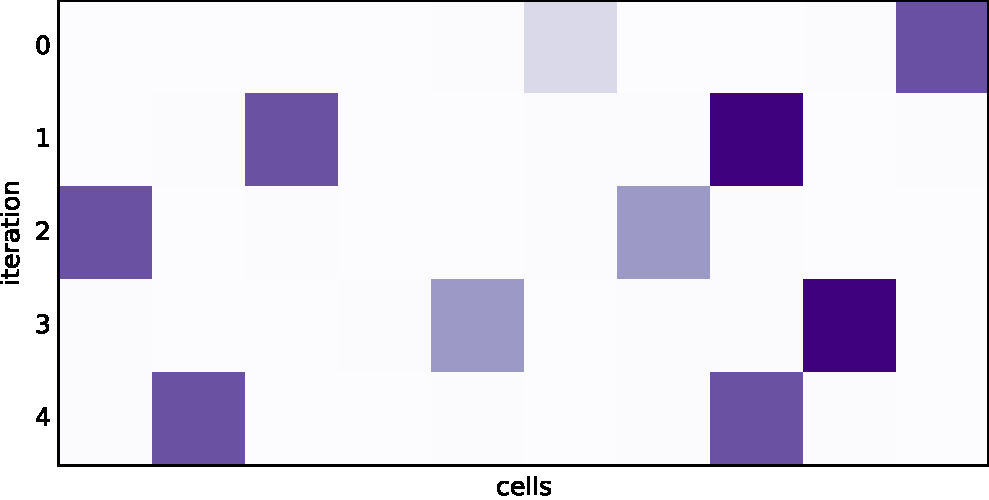
\includegraphics[width=.8\linewidth]{images/cellular-automata-based-sim}
	\caption{Ejemplo de un simulador de tráfico basado en autómatas celulares. En éste, el espacio se divide en celdas que pueden, o bien estar vacías, o bien ocupadas por un vehículo. La ilustración representa la evolución de los tiempos para cada vehículo (representado por un punto) según se desplaza a través del espacio discertizado en celdas de $7.5m$. Concretamente muestra la evolución a lo largo del tiempo del movimiento de un modelo de \textit{car-following} de tres vehículos. Fuente:~\cite{Brilon1999}.}
	\label{fig:cellular-automata-based-sim}
\end{figure}

En el caso del espacio, la clasificación diferencia las simulaciones que se mueven por un espacio discreto o por uno continuo:

\begin{itemize}
	\item De espacio \textbf{discreto}. Simulación donde el espacio está dividido en celdas que nosmalmente sólo pueden estar ocupadas por un elemento en un momento determinado. Este es el caso, por ejemplo, de los simuladores basados en autómatas celulares. La figura~\ref{fig:cellular-automata-based-sim} ilustra el comportamiento de uno de estos tipos de simulador.
	\item De espacio \textbf{continuo}. Simulación que transcurre en una secuencia infinita de puntos en el espacio. Es el caso por ejemplo de los simuladores basados en modelos lineales, como podemos ver en el ejemplo de la figura~\ref{fig:car-following-based-sim}.
\end{itemize}

En el caso del tiempo, la división se realiza en los mismos términos que en los del espacio:

\begin{itemize}
	\item De tiempo \textbf{discreto}. También denominada de \textit{simulación de eventos discretos}, divide el tiempo en intervalos discretos, generalmente (aunque existen excepciones) de longitud fija duranet toda la simulación. Los simuladores basados en autómatas celulares son también simuladores típicos discretos, ya que cada posición en el espacio se va calculando para cada intervalo discreto de tiempo (ver figuras~\ref{fig:cellular-automata-based-sim} y~\ref{fig:nagel-schreck}).
	\item De tiempo \textbf{continuo}. En estos simuladores el tiempo es un factor más para un modelo de ecuaciones diferenciales. La figura~\ref{fig:car-following-based-sim} ilustra un modelo de \textit{car-following} que puede implementarse en una smiulación de tiempo continuo si la aceleración viene determinada por un modelo que entre otros factores incluye el tiempo.
\end{itemize}

\begin{figure}
	\centering
	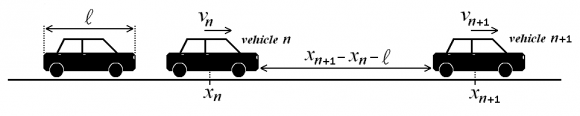
\includegraphics{images/car-following-based-sim}
	\caption{Ejemplo de un modelo lineal en un espacio continuo. La posición del vehículo es un valor $x \in \mathbb{R}$. Este ejemplo representa un modelo de \textit{car-following} donde el comportamiento de la aceleración del vehículo es determinado por la distancia al coche siguiente. Fuente:~\cite{Tordeux2011}.}
	\label{fig:car-following-based-sim}
\end{figure}

En nuestro caso, queremos conocer la situación exacta del vehículo y no una situación aproximada en una separación discreta del espacio. Esto nos dirige hacia simuladores de espacio continuo. Por otro lado, nosotros realizamos la recolección de datos en intervalos cuantificables de tiempo, los cuales serán usados para modelar los comportamientos de los conductores y para contrastar los resultados; por tanto, la elección está sesgada hacia simulación de tiempo discreto.

\section{Modelos de microsimulación}

Si bien es cierto que los sistemas de partículas son usados también para simulación de tráfico microscópico, su ámbito de aplicación es el mismo que el del punto de vista macroscópico, esto es, usar sistemas de partículas para el análisis del tráfico como fluido. Por ello como vertientes principales para representación del tráfico exploraremos los puntos de vista que se ocupan de éste desde el punto de vista del individuo: los autómatas celulares y los sistemas multiagentes.

\subsection{Microsimulación basada en autómatas celulares}

Un autómata celular es una colección ordenada de celdas o \textit{células} $n$-dimensionales que parcelan el universo en estudio. Cada una de dichas celdas se encuentra en un estado (e.g. contiene un valor numérico), y el estado de todas ellas se actualiza síncronamente (esto es, todas a la vez) en intervalos regulares de tiempo denominados \textit{ciclos}. El camio de estado de cada célula depende de los valores de las células vecinas y del algoritmo de modificación al que responden todas y cada una de las células.\sidenote{Hay realmente máquinas capaces de operar de esta manera, es decir, arquitecturas basadas en autómatas celulares. En ellas, cada ciclo de reloj actualiza todas las celdas de memoria del autómata. Éstas arquitecturas se suelen usar para la implementación de modelos físicos \TODO{buscar referencias}, superando en varios órdenes de magnitud la capacidad computacional de las arquitecturas tradicionales.}.

Estos modelos de microsimulación, debido a la propia naturaleza de los autómatas celulares, se encuentran clasificados como simuladores de tiempo y espacio discretos, y se usa debido a su facilidad de implementación y su eficiencia, ya que es fácilmente paralelizable.


\begin{figure}
	\centering
	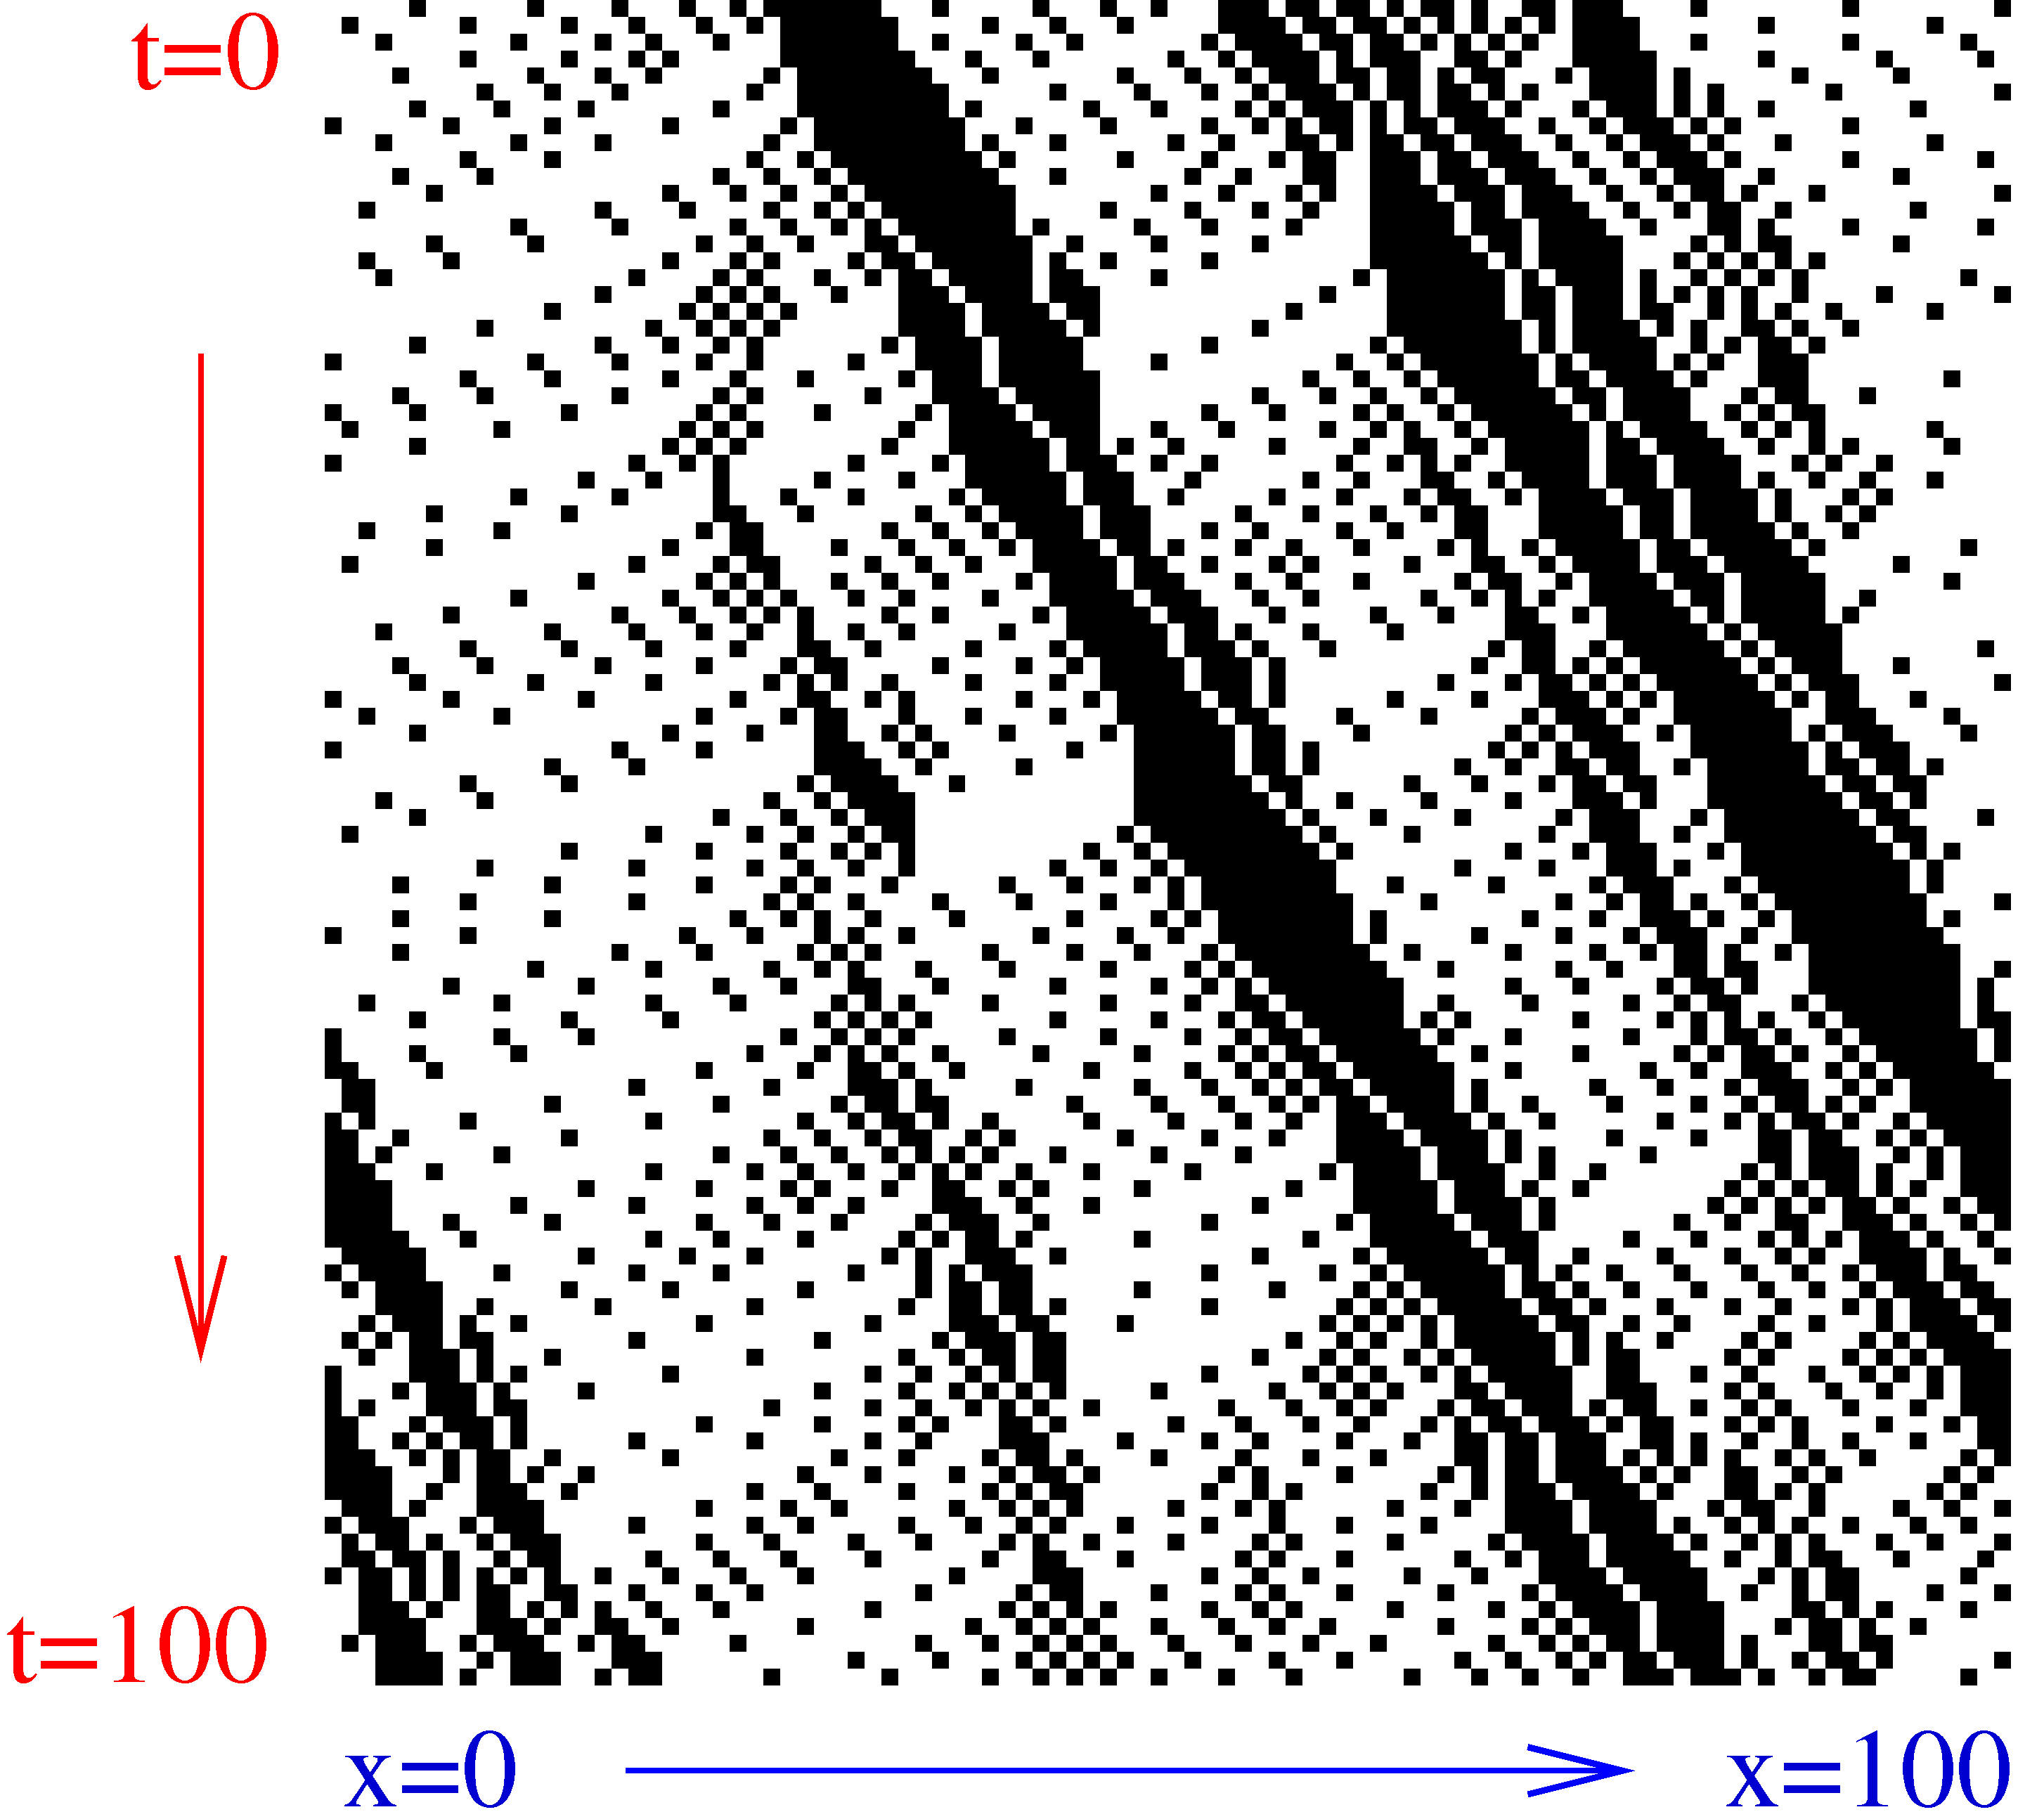
\includegraphics[width=.75\linewidth]{images/nagel-schreck}
	\caption{Representación de la evolución de un atasco en una autopista  de $100$ celdas de longitud usando el modelo Nagel-Scherckenberg. Con una densidad de ocupación $\rho = 0.35$ y una probabilidad de frenada de $p = 0.35$ se puede observar en la figura cómo se desplazan las olas del atasco a lo largo de los $100$ ciclos de la simulación. Feunte: Wikimedia}
	\label{fig:nagel-schreck}
\end{figure}

El modelo clásico de esta aproximación es el de Nagel-Scherckenberg (\cite{Nagel1992}), un modelo teórico creado para la simulación de tráfico en autopistas. La figura~\ref{fig:nagel-schreck} muestra la evolución del tráfico en una autopista a lo largo del tiempo de un autómata de este tipo. El resúmen de su funcionamiento es el siguiente:

\begin{itemize}
	\item La vía está divida en celdas de longitud $7,5m$ debido a que esta distancia es la media entre los parachoques traseros de dos coches consecutivos en un atasco.
	\item La celda puede tener dos estados, vacía o con un coche a una velocidad $v = \{0, \ldots, v_{max}\} \in \mathbb{N}$, esto es, discreta. La unidad de medida es $c/\Delta t$ siendo $c$ un número de celdas.
	\item $\Delta t$ queda establecido en $1s$, considerado el tiempo medio de reacción de un conductor ante una eventualidad. Esto hace, por ejemplo, que una velocidad de $6 c/\Delta t$ sea $45 m/s$ ($162 km/h$).
	\item En cada ciclo, se realizan cuatro acciones de manera simultánea: acelerar (nua unidad si no están a la máxmia velocidad), frenar (si se ven obligados en función de la velocidad y la distancia del siguiente vehículo), freno aleatorio (con una probabilidad de $p = 0.5$ la velocidad se reduce en una unidad hasta un mínimo de $v = 1 c/\Delta t$) y reposicionamiento (se avanzan tantas celdas como indica la velocidad.)
\end{itemize}

En general los modelos de la literatura suelen ser una variación de éste con ligeras modificaciones para estudiar aspectos concretos de modelos de tráfico, como la modificación del paso de \textit{aleatorización} (e.g. \cite{Barlovic1998}) o celdas más pequeñas (e.g. \cite{Krauss1997}) para comprobar la metaestabilidad del flujo de tráfico, o modelos y reglas para vías de dos carriles (e.g. \cite{Brilon1999} en la figura~\ref{fig:cellular-automata-based-sim} y~\cite{Nagel1998}).

\subsection{Microsimulación basada en sistemas multiagentes}

Los modelos basados en autómatas celulares, aunque interesantes, no son suficientemente realistas desde un punto de vista microscópico. Unos ejemplos: en una situación típica de un modelo Nagel-Scherckenberg, las posiciones de los vehículos se dan en últiplos de $7,5$ metros. Además, un vehículo realiza aleatoriamente aceleraciones y deceleraciones de $27 km/h$. Incluso en una situación favorable, cualquier vehículo puede realizar una aceleración de $0$ a $162km/h$ en sólo $6$ segundos. Por tanto, no ofrecen una visión fiable en caso de querer realizar estudios muy detallados del tráfico a nivel micro.

Los sistemas multiagentes ofrecen otro punto de vista a la simulación de tráfico dado que cada vehículo es modelado como un agente independiente. Este paradigma se ha desarrollado en detalle en la sección \ref{ch:sota-agents-and-mas:s:mas} del capítulo \ref{ch:sota-agents-and-mas}. Por ello en este apartado se explicará únicamente el por qué de la elección de este modelo describiendo sus ventajas frente a los sistemas basados en autómatas celulares.

Una de las principales razones por las que usar un sistema multiagente es que cada uno de los individuos o "agentes" tienen su propia entidad dentro del sistema. Esto es, perciben tanto el entorno como el resto de agentes y actúan de acuerdo a lo percibido y a su comportamiento preestablecido. Basarse no sólo en las magnitudes físicas del resto de vehículos (e.g. distancia, aceleración, \ldots) sino también en un comportamiento de conducción ofrece un interesante campo de estudio a nivel cognitivo.

Además, y a diferencia de los autómatas celulares, los sistemas multiagentes pueden emplazarse en un entorno virtual que represente un espacio continuo y no discreto. Esto permite modelar con mayor fidelidad magnitudes físicas asociadas a cada agente (e.g. posición y velocidades actuales, dimensiones del vehículo, masa, velocidad máxima permitida, \ldots).

Cada uno de los agentes es independiente del resto. Esta independencia da la posibilidad de tener todos los agentes diferentes entre sí. Aunque esto de por sí no tiene por qué tener demasiada utilidad, sí que lo tiene poder experimentar con diferentes perfiles de conducción (e.g. un perfil agresivo en un flujo de tráfico dominado por conductores tranquilos). Esto es debido a que en un sistema multiagente cada agente es una parte del sistema y las decisiones de cómo se ha de comportar un agente se toman desde el propio agente. Desde el punto de vista de un autómata celular, el comportamiento existe en cada celda, dando control parcial o nada de control al estado de cada celda.

Los estudios en materia de simuladores de tráfico con sistemas multiagente no se limitan a vehículos, sino que se usan también en áreas como el control de luces de tráfico o agentes para peatones entre otros. Un ejemplo es el estudio presentado en~\cite{Clymer2002} donde los agentes del sistema son las señales de tráfico luminosas y no los vehículos, y donde el objetivo es adaptar la señalización en una red de carreteras para minimizar al máximo el tiempo de espera por parte de los vehículos en las intersecciones gestionadas por las señales.

\begin{figure}
	\centering
	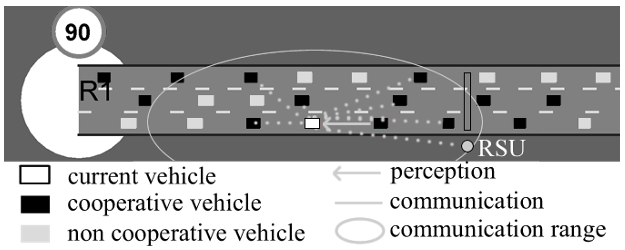
\includegraphics{images/cooperative-traffic-movsim}
	\caption{Captura de pantalla del simulador MovSim. Este simulador implementa un modelo multiagente donde los vehículos incorporan sistemas de comunicación vehicular. El estudio se centra en el uso de la comunicación entre vehículos para el acoplamiento dinámico de vehículos en sus respectivos carriles. Fuente: \cite{Gu2015}.}
	\label{fig:cooperative-traffic-movsim}
\end{figure}

Otra ventaja de este modelo es en el área de las comunicaciones extravehiculares (V2I) e intervehiculares (V2V). Es relativamente rápida la implementación de diferentes políticas y protocolos de comunicación via sensores y actuadores para estudiar estos tipos de redes de comunicación (ver figura~\ref{fig:cooperative-traffic-movsim}). En~\cite{Shiose2001}, por ejemplo, se hace uso de un sistema multiagente para implementar diferentes formas de comunicación intervehicular con el objetivo de aliviar congestinoe de tráfico. En el caso de redes extravehiculares, un buen ejemplo es~\cite{Dresner2004}, donde se representan como agentes tanto los vehículos como las intersecciones de la vía. Éstas gestionan un sistema de reservas que los vehículos que van a entrar en la intersección solicitan, gestionando  comunicando en todo momento mediante eventos los cambios en dicho sistema. El estudio concluye que una comunicación de este tiop es más eficiente que una intersección clásica basada en señales de tráfico luminosas.

\section{El vehículo como agente inteligente}

En nuestra tesis el trabajo se basa en la representación del comportamiento de un conductor. Para simplificar el problema asumiremos que los términos \enquote{conductor} y \enquote{vehículo} son equivalentes y que se refieren a la tupla \enquote{(vehículo, conductor)}.

No sé cómo ponerlo, pero esta información puede ser útil aquí. A lo mejor hay que separarlo, no sé. Yo lo pongo aquí porque me ha venido ahora.

\begin{itemize}
	\item \textbf{Percepción}. Característica intrínseca a todo ser vivo para la obtención de información del entorno. Pues para los agentes inteligentes, lo mismo. Puede ser en forma de sensores (e.g. sensor de velocidad, acelerómetro, sensor de distancia, lidar, cámaras, termómetros, gps, \ldots), conocimiento (e.g. controlador difuso, sistema experto, red neuronal, es decir, información procesada que ad valor añadido), datos GIS, comunicación con otros vehículos (e.g. V2V, V2E, \ldots). Un simulador nos ofrece estos sensores casi gratis, pero nuestro problema es que para la generación de modelos necesitamos previamente haber capturado información con dichos sensores y en físico ya es otra cosa.
	\item \textbf{Toma de decisiones}. Un agente racional en un sistema multiagente ha de ser capaz de razonar acerca del mundo, de su propio estado y del estado del resto de agentes.
	\item \textbf{Actuación}. La actuación es la consecuencia natural de las anteriores características. Dado un estado del mundo y un proceso cognitivo surgen acciones a realizar, tras las cuales se llega a un nuevo estado del entorno que provee de información actualizada para seguir actuando.
\end{itemize}

\section{Elección de software para las simulaciones}

En este apartado se facilita la comparativa realizada para la elección de simulador sobre el que basar los escenarios a plantear en las simulaciones de los modelos de conductor.

Hoy en día existe una oferta muy amplia de simuladores en el mercado, cada uno implementando uno o varios modelos diferentes y bajo diferentes licencias.

Cada simulador tiene sus ventajas e inconvenientes, y es por ello importante realizar un estudio previo para conocerlos y no llevarse sorpresas una vez se llega a estadios más avanzados del estudio. No se trata de realizar una comparativa en busca del mejor simlador de tráfico del mercado, sino en encontrar el simulador que más se adecúa a los criterios concretos para los propósitos de esta tesis.

\subsection{Entornos de simulación a estudiar}



El siguiente listado muestra la lista de simuladores de tráfico sobre los que se realizarán las comparativas. Por motivos de espacio no se han incluido todos los simuladores encontrados en la listeratura, sino que se han seleccionado únicamente aquellos que (i) aun existen y se pueden adquirir, y (ii) son entornos de microsimulación.

\begin{enumerate}
	\item \textbf{AIMSUN}. Entorno de simulación de granularidad micro, meso y macro desarrollado por la empresa \textit{Transport Simulation Systems}. Url: \url{http://www.aimsun.com/}.
	\item \textbf{TSIS-CORSIM}. Entorno de microsimulación compuesto de dos simuladores para distintos modos de tráfico (NETSIM para entornos urbanos y FRESIM para entornos interurbanos) desarrollado dentro de la Universidad de Florida por el centro \textit{McTrans}. Url: \url{http://mctrans.ce.ufl.edu/featured/tsis/}.
\end{enumerate}

Simuladores de pago:

Quadstone paramics (microscopic)
VISSUM (macroscopic)
VISSIM (microscopic)
ARCHISIM

Simuladores gratuitos:

Matsim
SUMO (microscopic)
Repast
MAINSIM
Synchro

Ni puta idea:

CUBE
SATURN
PARAMICS
TRANSIMS


\subsection{Criterios de selección}

Los criterios se muestran ordenados alfabéticamente:

\begin{enumerate}
	\item \textbf{Activo}. Si el simulador está activaemnte desarrollado o si por el contrario se trata de un proyecto con poca actividad por parte de sus autores. Es interesante hacer uso de un simulador que esté siendo activamente desarrollado porque eso favorece la aparición de parches y mejoras sobre el software.
	\item \textbf{Extensibilidad}. Si el simulador permite extender sus funcionalidades de alguna manera. Aunque se puede considerar que si es Open Software, es posible modificar su comportamiento para adcuarlo a los modelos desarrollados, es mejor que el propio software ofrezca los mecanismos necesarios para la integración sin necesidad de tocar el núcleo.
	\item \textbf{Granularidad}. Si el simulador es de tipo micro, meso o macro. Para nuestras necesidades es necesario un simulador que implemente microsimulación, ya que es el único tipo de granularidad que permite evaluar el comportamiento de un conductor independientemente del resto de la simulación.
	\item \textbf{Licencia}. Especifica con qué tipo de licencia se distribuye el software. Es preferible una licencia de tipo Open Software (\TODO hay que ver si esto está bien dicho o no) ya que de esta manera es posible modificar el software en caso de encontrar algún error o falta de funcionalidad que el fabricante no tenga pensado codificar.
	\item \textbf{Sistema operativo}. Sobre qué sistemas operativos está soportado el entorno de simulación. Es imprescindible que el software se ejecute sobre sistemas operativos GNU/Linux por la configuración de los sistemas sobre los que se trabaja, aunque es interesante también su funcionamiento en entornos tipo OS-X.
	\item \textbf{Tipo de simulación}. Qué modelo interno usa el motor para la simulación (e.g. automatas celurares, sistemas multiagentes, ...).
	particle system simulation).
\end{enumerate}

\subsection{Comparativa}

Al haber tal cantidad de simuladores, la comparativa se ha realizado descartando aquellos simuladores que no cuentan con características necesarias o que son de una tipología no deseada. A continuación se enumera la lista de razones por las que se han descartado simuladores junto con aquellos afectados por la decisión:

\begin{enumerate}
	\item Debe ser (o al menos soportar) un entorno de microsimulación.
	\item Debe ofrecer un entorno de simulación de tráfico general, no sólo casos particulares como congestión o colisiones.
	\item \ldots
\end{enumerate}

\begin{center}
	\footnotesize
	\begin{tabular}{lllll}
		\toprule
		& Aimsun & \acrshort{sumo} & TSIS-CORSIM & \\
		\midrule
		Activo & sí & sí & sí & \na \\
		\addlinespace
		Extensibilidad & \na & sí & no & \na \\
		\addlinespace
		Granularidad & & & & \\
		\quad Micro          & sí     & sí             & \na  & \na \\
		\quad Meso           & sí     & no             & \na  & \na \\
		\quad Macro          & sí     & no             & \na  & \na \\
		\addlinespace
		Licencia & & & & \\
		\quad Propietaria    & sí     & sí             & \na  & \na \\
		\quad Open Software  & no     & no             & \na  & \na \\
		\quad Compatible GPL & no     & no             & \na  & \na \\
		\addlinespace
		Sistema operativo & & & & \\
		\quad GNU/Linux      & sí     & no             & \na  & \na \\
		\quad OS X           & sí     & no             & \na  & \na \\
		\quad Windows        & sí     & sí             & \na  & \na \\
		\addlinespace
		Tipo de simulación   & \na    & \acrshort{mas} & italics & upright, caps \\
		\bottomrule
	\end{tabular}
\end{center}

\subsection{Entorno seleccionado: \acrshort{sumo}}

En definitiva, el simulador que más se adapta a nuestras necesidades y el que se usará como simulador base en el desarrollo de esta tesis será \gls{sumo}\sidenote{Sus principales publicaciones son~\cite{krajzewicz2002sumo}, \cite{behrisch2011sumo} y \cite{krajzewicz2012recent}.}. \gls{sumo} es un entorno de microsimulación de código abierto\sidenote{Licenciado bajo la \gls{gpl}, concretamente la versión $3.0$.} que implementa un modelo discreto en el tiempo y continuo en el espacio.

Además de simulación clásica, \gls{sumo} provee de una interfaz gráfica (se puede ver un pantallazo en la figura~\ref{fig:sumo-simulator}) donde se puede ver el comportamiento de cada vehículo durante la simulación. Es interesante para obtener de un vistazo información acerca del funcionamiento del modelo en concreto a controlar. Otras de las características que el simulador ofrece son las siguientes:

\begin{figure}
	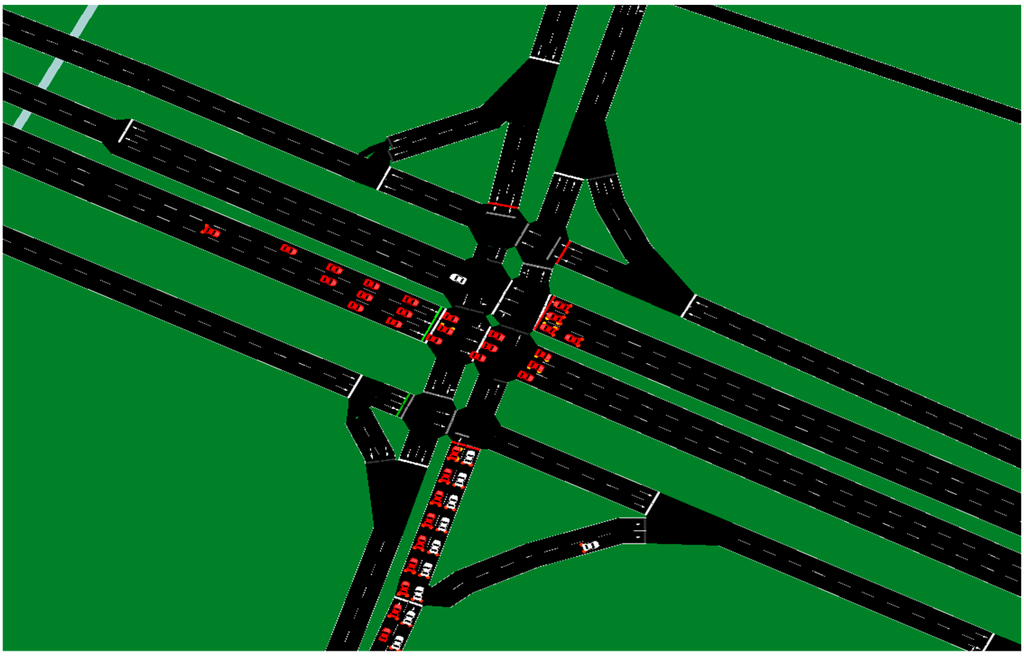
\includegraphics{sumo-simulator}
	\caption{Ejemplo de pantalla del simulador \gls{sumo}. Además de entorno de simulación propiamente dicho, \gls{sumo} provee de una interfaz gráfica que permite una visualización general, de zonas y de elementos en concreto a la vez que permite la variación de configuración de la simulación durante el desarrollo de la misma.}
	\label{fig:sumo-simulator}
\end{figure}

\begin{itemize}
	\item Multimodalidad permitiendo modelar no sólo tráfico de vehículos sino de peatones, bicicletas, trenes e incluso de barcos.
	\item Vehículos de diferentes tipologías, Simulación con y sin colisiones de vehículos.
	\item Diferentes tipos de vehículos y de carreteras, cada una con diferentes carriles y éstas con diferentes subdivisiones de subcarriles (diseño conceptual para permitir las simulaciones )
\end{itemize}

Al estar licenciado bajo la licencia \gls{gpl}, su distribución implica a su vez la distribución de su código fuente. Esto permite la modeificación de su comportamiento y el desarrollo de nuevos modelos integrados dentro del simulador. Sin embargo nosotros no haremos uso de esta característica, sino que usaremos \gls{sumo} como aplicación servidor y el módulo \gls{traci} como aplicación cliente desde donde gestionar todos los aspectos de cada simulación.

\subsection{La interfaz \glsentrylong{traci}}
\chapter{Modelos de comportamiento}
\label{ch:sota-behavior-models}

En un simulador de tráfico que basa su funcionamiento en un modelo micro de múltiples agentes haciendo las veces de conductores, el comportamiento de éstos es crucial para que éste describa su evolución de nua manera veraz, lo más aproximada a un sistema de tráfico real. Por ello, el conductor ha de ser diseñado teniendo en cuenta que ha de actuar tanto con el vehículo (en mayor o menos detalle) y su entorno (e.g. el resto de conductores, señales de tráfico, siste)
driver  has  to  be  designed  to  interact  with  other  dr
ivers,  traffic  signals,  pedestrians  and  ITS 
systems.

A lo largo de los años se han estudiado diferentes modelos de comportamiento de conductor. Éstos suelen caer dentro de dos categorías principalmente, el \textbf{car-following} o \textit{seguimiento de vehículos} que se ocupa de determinar el comportamiento de un vehículo en función del comportamiento del inmediatamente siguiente y el \textbf{lane-changing} o \textit{cambio de carril} que estudia la forma en la que un conductor decide realizar un cambio de un carril origen a un carril destino. Y aunque tradicionalmente se han tratado como dos modelos independientes y ha sido estudiado más el primero que el segundo desde los años 1950, en los últimos 20 años se ha tendido a modelar ambos problemas como un único mecanismo~\cite{Ma}.

La mayoría de los modelos basan su funcionamiento en técnicas pertenecientes al \acrlong{hc} o lo que es lo mismo, están basados en fórmulas matemáticas y reglas de la lógica convencional con parámetros que se ajustan a partir de la observación de datos reales. No son los único modelos que existen, ya que en los últimos años ha empezado a crecer el interés por las técnicas de la \ac{ci} en el campo y por tanto existen ciertos estudios de técnicas más acorde con este punto de vista. En éstas es en las que nos centraremos en este capítulo, el cual desarrollará qué entendemos por comportamiento en conducción y qué modelos de interés dentro de la \ac{ci} se han desarrollado hasta ahora.

\TODO{Creo que en lugar de separar en lane-changing, car follownig y sucesivos, habría que explicarlos y luego en un apartado más adelante revisar el estado del arte en comportamientos.}

\TODO{Quizá tiene sentido especificar aquí que va a ser como DVU, es decir, 1 vehículo=1 conductor=1 agente.}

\section{Comportamiento en la conducción}

¿A qué nos referimos cuando hablamos del "comportamiento"? Según el diccionario de la real academia, \enquote{comportar} se define como \textit{actuar de una manera determinada}. Sin embargo, no queda claro qué factores constituyen el comportamiento al volante.

Atendiendo a la literatura, \TODO un par de párrafos para hablar de comportamiento

¿Cómo se define el comportamiento de un conductor?

En~\cite{michon1985critical} describen la conducción como una trea separada en $3$ niveles jerárquicos, el de estrategia, el de maniobra y el de control. En la figura~\ref{fig:three-levels-of-human-driving}. se ve mejor.
\begin{figure}
	\centering
\smartdiagram[descriptive diagram]{
	{$3$, {\textbf{Estrategia} (e.g. planificación de la ruta, \ldots})},
	{$2$, {\textbf{Maniobra} (e.g. cambio de carril, \ldots})},
	{$1$, {\textbf{Control} (e.g. cambio de marcha \ldots)}},
}
	\caption{Los tres niveles jerárquicos que describen la tarea de conducción según~\cite{michon1985critical}: \textit{estrategia} (i.e. las decisiones generales), la \textit{maniobra} (i.e. decisiones durante la conducción de más corto plazo) y \textit{control} (i.e. comportamientos automáticos). (\TODO{Hacer mejor esta figura})}
	\label{fig:three-levels-of-human-driving}
\end{figure}

SUMO usa (al menos así lo indican en el paper del 2002) el modelo Gipps\cite{krajzewicz2002sumo}. No sé si ellos han hecho una extensión del modelo o están referenciando la extensión y ellos sólo la implementan. En el paper del 2012 citan que el modelo car-following que usan por defecto es el desarrollado por Stefan Krauß\cite{jin2016evaluation}, debido a su simplicidad y su velocidad de ejecución.

El modelo ha probado ser válido, pero tiene algunos defectos, por lo que existe un API para implementar otros modelos. En la actualidad están incluidos en el sistema los modelos IDM\cite{treiber2000congested} (\textit{Intelligent Driver Model}), el modelo de tres fases de Kerner\cite{kerner2008testbed} y el modelo de Wiedemann\cite{wiedemann1974simulation}.

La práctica totalidad de modelos para el comportamiento de conductores en tráfico se basan en una estructura jerárquica de control\cite{michon1985critical}. Por lo que veo este paper es de 1985, así que afirmar eso 30 años después es una barrabasada. Hay que buscar algo más para apoyar eso o para indicarlo como una anécdota.

En el paper \cite{al2001framework} describen un framework para la modelización de comportamiento de conductores dentro de simuladores.

En~\cite{tang2014new} los autores proponen un modelo de car following teniendo en cuenta comunicación entre vehículos.

\TODO Hoy he descubierto que hay una cosa que se llama naturalistic traffic study o naturalistic traffic observation (\gls{nds}) que es un estudio naturalístico, es decvir, observar en el mundo real con detalle y extraer datos de ello. A lo mejor hablando así queda como más profesional :D.

Los \gls{nds} basan su funcionamiento en la captura masiva de datos de conducción, normalmente involucrando una gran cantidad de sensores, para analizar el comportamiento del conductor, las características del vehículo, la vía, etcétera. La cantidad de sensores y la velocidad de captura hacen que la tarea de analizar y extraer conclusiones  sea una tarea prácticamemte imposible para un humano, por lo que es necesario el uso de técnicas de análisis de datos que suelen recaer en los campos de la estadística y del aprendizaje automático.

En~\cite{sekizawa2007modeling} describen modelos supervisados offline para capturar el comportamiento del conductor basados en auto-regresión a trozos. Más adelante lo extienden en~\cite{terada2010multi}, aunque los datos de entrenamiento son extraídos directamente de simulaciones, no del \enquote{mundo real\textsuperscript{TM}}.

En~\cite{bando2013unsupervised} describen otro modelo no supervisado offline basado en un modelo bayesiano no paramétrico para la clusterización, combinado con un LDA (Latent Dirichlet Allocation, sea lo que sea esto) para la clusterización a más alto nivel. (\TODO ¿este método usa datos reales?)

Estos trabajos (\cite{sekizawa2007modeling}, \cite{terada2010multi} y \cite{bando2013unsupervised}) tienen la desventaja de ser computacionalmente muy costosos y con poca precisión en el caso de variar mucho los escenarios de entrenamiento y de test.

En~\cite{maye2011bayesian} se presenta un modelo online donde se infiere el comportamiento del conductor haciendo uso de una IMU (Intertial Measurement Unit) y una cámara. Primero de la IMU se sacan datos que se separan en fragmentos para luego relacionarlos con las imágenes obtenidas de la cámara. (\TODO ¿Hacia dónde mira la cámara?). Los modelos propuestos en~\cite{johnson2011driving} y~\cite{van2013driver} también se apoyan en el funcionamiento de clasificar las segmentaciones de una IMU, pero con técnicas distintas y sin cámara (\TODO Que digo yo, ¿qué clasifican exactamente? es más, dependiendo de qué clasifican, para qué vale la camarita del~\cite{maye2011bayesian}?). Además hacen uso de señales externas y umbrales de activación para hacer más efectiva la clasificación (\TODO corroborar).

En el artículo~\cite{bender2015unsupervised} se usa también un modelo no supervisado online con una aproximación bayesiana para identificar los puntos de cambio sin depender de parámetros externos (e.g. umbrales o señales). Se basa también en (1) segmentar los datos de conducción y (2) asignar estos datos a clases que se corresponde n con comportamientos de conducción. Tiene la ventaja de ser más eficiente y rubusto que los anteriores.

La idea de estos métodos desde el~\cite{sekizawa2007modeling} hasta el~\cite{bender2015unsupervised} creo que es el de un sistema que traduzca datos en crudo a datos de más alto nivel. Esto es debido a que la cantidad de datos que se pueden generar en un sólo coche (no digamos ya una flota de ellos) es tan grande que para determinados sistemas disponer de información de más alto nivel haría más sencillo su desempeño (por ejemplo, \gls{adas} que funcionasen con datos de \enquote{adelantando} que sus valores de giro, aceleración en una ventana temporal).

En~\cite{satzoda2013towards}, haciendo uso de la información combinada de bus CAN, cámaras, GPS e información digitalizada el mapa donde se circula se determina una amplio abanico de información crítica en diferentes condiciones de la carretera. La información que sacan es: número de cambios de carril a la derecha, a la izquierda, tiempo en autopista y carretera urbana, distancia recorrida, velocidades medias en autopista y urbano, paradas, giros a la derecha, a la izquierda, incormporaciones y salidas de autopsta, tiempo gastado en un sólo carril, curvas a la izquierda, curvas a la derecha y distancia media al carril central

En~\cite{al2001framework} describen un framework para la modelización de comportamiento de conductores dentro de simuladores. Se basa en cuatro unidades de funcionamiento interconectadas, la de percepción (percibe el entorno en términos locales y globales), la de emoción (cómo responde emocionalmete al entorno), la de decision-making (investiga posibles acciones que podrían servir a las necesidades del módulo emocional) y la de decision-implementation (intenta implementar las decisiones cuando emergen condiciones de tráfico lo suficientemente seguras para llevarlas a cabo). Tengo que volver a leerlo después de hacer una primera introducción en el tema de agentes, porque me parece poner nombrecitos a un tipo de agente que funciona de esa misma manera, pero lo mismo no.

En~\cite{terroso2015complex} analizan lo que ellos denominan el concepto del \gls{ivca}, lo que viene a ser el contexto definido \textbf{dentro} del vehículo, llegando a intentar predecir no sólo el número de ocupantes (ese es un problema sobradamente superado) sino la tipología o clase de ocupante (e.g. niños, adultos, ... \TODO buscar cuáles son las tipologías). Para ello hacen uso de un \gls{cep}\footnote{Un \gls{cep} es un método por el cual se lee un flujo de información compuesta de flujos de distintas fuentes (de ahí el \textit{complex}) para detectar eventos o patrones que pueden indicar la presencia de situaciones a analizar lo más rápido posible.} para procesar los datos de los diferentes sensores del vehículo y así detectar y analizar patrones característicos.

El artículo~\cite{munoz2010human} es muy interesante ya que para la competición \textit{2010 Simulated Car Racing Championship} desarrollaron un controlador no para minimizar el tiempo en realizar las carreras, sino para hacerlo lo más parecido posible a cómo se comporta un humano. Para ello hicieron uso de redes neuronales para calcular trayectorias y de un proceso de aprendizaje a partir de información extraída de un conductor real en el simulador \gls{torcs}.

Aunque \gls{torcs} es usado como entorno de simulación en diversos concursos e investigaciones, se trata de un juego, y es que los juegos son un sandbox perfecto como entorno de simulación, ya que presentan una abstracción del dominio sobre el que trabajar. Otros trabajos en esta línea (entrenamiento de redes neuronales en este simulador) son los de~\cite{munoz2009controller} y~\cite{van2009robust}, el primero entrenando perceptrones multicapa (\TODO verificar) con un backpropagation haciendo uso de un dataset proporcionado por un bot y otro haciendo uso de un algoritmo evolutivo multiobjetivo para optimizar la red de acuerdo a un conjunto de datos proporcionado por un conductor real. Sin embargo, este tipo de modelos se encuentran más cercanos al nivel de control que al nivel de maniobra descritos en la figura~\ref{fig:three-levels-of-human-driving}.

En~\cite{van2013driver} hacen uso de os sensores de inercia de un coche (a saber qué coche tienen) para construir un perfil de conductor. Concluyen que frenar y girar caracterizan mejor a los conductores frente a acelerar.

\section{lane change y car following}

MOBIL --> http://www.traffic-simulation.de/MOBIL.html, http://www.mtreiber.de/publications/MOBIL\_TRB.pdf y http://link.springer.com/chapter/10.1007\%2F978-3-540-77074-9\_19\#page-1

\section{car-following}

En un modelo de tipo car-following los vehículos están representados por una tupla del estilo $(x_n, v_n, a_n, t_n)$ donde $x_n$ es la localización espacial, $v_n$ la velocidad, $a_n$ la aceleración y $t_n$ el momento en el tiempo del vehículo $n$. El modelo es una serie de reglas o ecuaciones que actualizan estos valores a lo largo de $t_n$. Cambiar la definición a algo que sea más claro o citar esta que sale en~\cite{Aghabayk2015}.

En~\cite{Aghabayk2015} realizan un estado de la cuestión en materia de modelos de tipo car-following. El autor divide en dos categorías los modelos, los clásicos y los basados en inteligencia artificial.

\begin{enumerate}
	\item \textbf{Clásicos}. Son aquellos modelos donde la acción que realiza el vehículo viene determinada por una o más ecuaciones en función de las acciones que toma el vehículo delantero. Se pueden considerar limitados porque se centran en los resultados del comportamiento y no en el comportamiento en sí. Además se basan en que determinadas variables (e.g. tiempo de reacción) son las mismas para cada conductor.
	\begin{enumerate}
		\item \textbf{De estímulo-respuesta}. La respuesta está directamente relacionada con el estímulo creado por el comportamiento del coche de delante, generalmente una respuesta de tipo aceleración o deceleración aplicada con un pequeño retardo $t$. Los métodos de esta clase de modelo ssuelen ser sencillos, pero tiene dos problemas principales, (i) que los modelos no capturan los comportamintos de diferentes tipos de conductores o vehículos y (ii) supone que el conductor es capaz de observar los más mínimos cambios en el coche delantero cuando esto en realidad no es así (4-7).
		\item \textbf{De distancia segura}. También denominados de prevención de colisión, basan su funcionamiento en dejar una distancia segura entre el coche delantero y el actual. El principal problema de estos modelos es que no se corresponden con la realidad, ya que un conductor obtiene información de muchas más fuentes y reaccionan en consecuencia y por tanto el comportamiento exhibido en estas simulaciones no se corresponde con el comportamiento real~\cite{Pipes1953}.
		\item \textbf{De avance deseado}. Similares al anterior, estos modelos basan su funcionamiento en tratar de mantener una distancia entre el parachoces trasero del coche frontal y el coche actual. Como en el caso anterior, este modelo no modela corectamente el comportamiento de un conductor debido a que hay muchos parámnetros que no se miden para determinar la distancia a mantener en cada momento.
		\item \textbf{Psicofísicos}. En este modelo, la suposición es que un conductor es capaz de detectar los cambios de velocidad en el vehículo frontal a partir del cambio en el ángulo visual con éste (8-10).
	\end{enumerate}
	\item \textbf{Basados en \acrlongsp{ai}}. Son todos aquellos modelos que están basados en técnicas del campo de la \acrshort{ai}.
\end{enumerate}

Nosotros nos centramos en \acrshort{ai}, seguramente haya que recortar un poco lo de arriba para nombrarlo por encima. Quizá apuntando a los distintos tipos y ya. Según~\cite{Aghabayk2015}, los modelos basados en \acrlongsp{ai} funcionan en base a dos técnicas principalmente, las \acrlongplsp{ann} y la \acrlongsp{fl}.

\subsection{Modelos basados en lógica difusa}

Los modelos de car following que se basan en la lógica difusa suelen apoyarse en la convicción de que la información que maneja el conductor a la hora de tomar decisiones proviene de un análisis no demasiado detallado de la situación que le rodea, y que por tanto que su razonamiento parte de conceptos imprecisos y vagos que llevan a una respuesta no demasiado bien definida.

\cite{Kikuchi1992} fueron los primeros en aplicar lógica difusa a modelos de conducción. Usaron el modelo GHR (\cite{Chandler1958}). Las entradas al modelo eran distancia al coche delantero, diferencia de velocidades, aceleración y deceleración del coche delantero. La aceleración y deceleración se toman como entradas diferentes porque postulaban que el comportamiento antes ambos casos era diferente (aunque creo que esto es equivalente a usar particiones no simétricas de la variable lingüística. Como salida, la aceleración/decelearación del coche actua

Otros trabajos que trabajan con lógica difusa: (Chakroborty y Kikuchi, 1999, 2003; Das, Bowles, Houghland, Hunn y Zhang, 1999; Gao, Hu, y Dong, 2008; Gonzalez-Rojo, Slama, Pereira y Mora-Camino, 2000, 2002; Hatipkarasulu y Wolshon, 2003; McDonald et al., 1997; Rekersbrink, 1995; Won, Lee, Lee, y Kim, 2007; Zheng y McDonald, 2005, Wu, Brackstone y McDonald, 2003). Ninguno de estos estudios considera diferentes tipologías de vehículos para el car following

Problemas:

\begin{enumerate}
	\item ¿Qué reglas usan los humanos para modelar su comportamiento? Desconocerlas implica modelos no realistas. En (Wu, Brackstone, y McDonald, 2003) intenta suplir este problema con encuestas a conductores.
	\item Los problemas inherentes de los controladores difusos. ¿Cómo validar las funciones de pertenencia? ¿cómo determinar las reglas difusas?
\end{enumerate}

\subsection{Modelos basados en redes neuronales artificiales}

Las redes neuronales se han aplicado mucho sobre el campo de las ITS en general, y sobre la conducción autónoma y el análisis del comportamiento de los conductores (Dougherty, 1995).

En (Fix y Armstrong, 1990) implementaron un controlador basado en redes neuronales para al comportamiento del car following en un microsimulador entrenando dicho modelo previamente con datos extraídos de un conductor en dicho simulador.

En (Dougherty, Kirby y Boyle, 1993) usan redes para determinar el nivel de congestión en la vía.

(Hongfei, Zhicai y Anning, 2003) son los primers en usar datos reales de un coche instrumentado usando el método Five-Wheel-System, que está especificado en su paper de aquella manera y que no me entero de nada. A partir de las entradas correspondientes a velocidad relativa, espacio relativo, velocidad y velocidad deseada (para ello, clasifican al conductor de agresivo, normal, conservador) determinan la aceleración/deceleración del vehículo. No lo aplican a ningún simulador, sólo que los valores se ajustan.

(Panwai and Dia, 2007) redes neuronales usando el dataset de (Manstetten, Krautter y Schwab, 1997) desarrollan una red neuronal para mantener la distancia con el siguiente vehículo. Este modelo sí se evaluó en el simulador AIMSUN, y los resultados muestran una buena correspondiencia entre los datos y la realidad. No replica sin embargo el comportamiento de frenar hasta parar o de acelerar desde parado.

Problemas:

\begin{enumerate}
	\item Es imposible determinar por qué la red funciona como está funcionando.
	\item Los clásicos de los problemas de redes, el no aprendizaje y la especialización.
\end{enumerate}

\subsection{Otras técnicas}

\subsection{Aproximaciones híbridas}

(Li, 2003) y (Ma, 2004) usan aproximaciones de fuzzy neural networks y neurofuzzy respectivamente. No proveen sin embargo de documentación y no se investiga la aplicación de estos modelos a microsimuladores de tráfico.

(Aghabayk, Forouzideh y Young, 2013) usan el modelo de árboles lineales locales (LOLIMOT, (Nelles, 2001)) que no deja de ser una aproximación neuro-fuzzy del comportamiento. Intenta incorporar imperfecciones perceptuales en un modelo de car following. El modelo está basado usando datasets reales y los resultados indican que se ajusta lo predicho con la realidad, pero no hay pruebas realizadas en microsimuladores.

En~\cite{Ma}, bajo la suposición de que el ser humano toma múltiples decisiones relacionadas basándose en su percepción (imprecisa) del entorno propone un método masado en un sistema de inferencia difusa para tomar decisiones tanto para el problema del \textit{car following} como para el del \textit{lan changing}, calibrando y ajustando dicho controlador mediante el uso de redes neuronales (aproximación Neuro-Fuzzy).



\section{lane-changing}

(Gipps, 1986, A Model for the Structure of Lane-Changing Decisions) propone un framework para el problema de cambio de carril que incluye numerosos factores, entre ellos señales de tráfico, tipos de vehículo (e.g. camiones) o \enquote{urgencia} en el camio de carril (e.g. proximidad a una salida o giro). El pricipal problema de las reglas de este modelo es que asumen que el cambio de carril ocurre sin forzar a los vehículos del carril de destino a modificar su comportamiento como disminuir la velocidad o parar.

En (Fritzsche, 1994, A model for traffic simulation) se describe un modelo de microsimulación para analizar cuellos de botella (e.g. un accidente donde se bloquea uno de los carriles). Es un caso típico donde los vehículos no pueden cambiar de carril sin la participación activa del resto de vehículos (colaboración). El modelo lo describe de una maera muy sucinta y no zonsidera comportamiento colaborativo en el cambio de carril.

Yousif and Hunt (1995) developed a microscopic simulation model for the investigation of lane changing behaviour on multi-lane unidirectional roadways. The rules pertaining to the desire and the possibility to change lane are based on similar logic to that described by Gipps (1986). Again, the assumption of the model is that if the available gap in the target lane is smaller than a given acceptable limit, no lane changing will take place. The main concern of the study is the relationship between lane utilisation and traffic flow on dual-carriageway roads under normal flow conditions (i.e. without incidents) and the model is adequate for this purpose. However, it could not produce realistic results when incidents or lane closures affect the flow conditions.

(Barcelo et al., 1996, PETRI: A parallel environment for a real-time traffic management and information system) describen el simulador AIMSUN. El comportamiento de cada vehículo en la simulación es modelado a través de múltiples modelos de comportamiento (e.g. car following, lane changing, gap acceptance). El modelo de cambio de carril es el usado en el modelo de Gipps, aunque el propio simulador permite la modelización de incidentes por lo que debe existir alguna variación del modelo original o un nuevo modelo para ese caso concreto.

(Wagner et al., 1997, Realistic multi-lane traffic rules for cellular automata) describe \enquote{un modelo de microsimulación mínimo para traproducir características macroscópicas en el flujo de tráfico}. El objetivo: definir reglas realísticas para modelar el cambio de carril usando carreteras con múltiples carriles. Para el cambio de carril, describen una serie de reglas para describir \enquote{cuando} cambiar de carril, y una \enquote{regla restrictiva de seguridad} que especifica que un coche que quiere cambiar de carril no moleste al coche de detrás en el carril objetivo. El modelo fue capaz de reproducir de forma satisfactoria las características de uso de los carriles en carreteras de múltiples carriles con diferentes flujos de tráfico sobre condiciones normales (i.e. sin incidentes) de tráfico.

En (Hunt and Lyons, 1994, Modelling of dual-carriageway lane-changing using neural networks) desarrollan un modelo de decisión usando redes neuronales. El modelo funciona a partir de presentarle una entrada visual del entorno alrededor del vehículo que quiere cambiar de carril. Sin embargo, no considera la cooperación entre vehículos.

En (Yang and Koutsopoulos, 1996, A Microscopic Traffic Simulator for Evaluation of Dynamic Traffic Management Systems) presentan el simulador MITSIM, desarrollado por el MIT (creo) en el que se habla específicamente de comportamiento colaborativo en cambio de carriles haciendo uso de lo que denominan "courtesy yielding function" (algo así como función de cesión de paso de cortesía), la cual se usa para para hacer espacio al vehículo que va a incorporarse al carril. Sin embargo, los detalles de dicho proceso no están especificados en el paper.

En (Modelling lane changing and merging in microscopic traffic simulation, 2002) (simulador SITRAS) dicen que según el comportamiento de (Gipps, 1986), el cambio de carril no ocurre nunca en una situación de congestión, y por tanto en este tipo de situaciones el vehículo tiene que forzar su movimiento hacia el carril. Como la interacción entre conductores en ese tipo de maniobras requiere comportamiento complejo de toma de decisiones, éstos pueden ser modelados con técnicas de agentes autónomos. También aquí hablan de los DVOs (driver-vehicle objects). Tienen características individuales como (i) tipo de vehículo, (ii) magnitudes físicos (tamaño, velocidad máxima, ...), (iii) tipo de conduictor y (iv) nivel de conocimiento de la red (porque afecta en la elección de ruta). Tienen un objetivo, llegar del origen al destino tan rápido como puedan. Esto implica un conjunto de decisiones a hacer en intervalos periódicos durante su funcionamiento (i) selección de ruta cada vez que se entra en un nuevo tramo y (ii) cálculo de la aceleración en cada intervalo).

En (Chaib-draa and Levesque, 1996, ) proponen un framework para trabajar con tres tipos diferentes de situaciones (rutina, familiar y no familiar) en sistemas multiagente, demostrando la aplicación en escenarios de microsimulacinó urbana). Su modelo se basa en una estructura jerárquica definida por los niveles de comportamiento humano y de técnicas de razonamiento propuestas por (Rasmussen, 1986, ) (skill-rule-knowledge). El comportamiento basado en habilidades (skills) se refiere a las actividades completamente automatizadas (percepción--ejecución) usadas típicamente en situaciones rutinarias. comportamiento basado en reglas se refiere a situaciones esteorotipadas (percepción--reconocimiento de la situación--planificación--ejecución) aplicable en su mayoría en situacionesfamiliares. El comportamiento basado en el conocimiento se refiere a actividades conscientes que implican trabajo de resolución de problemas y toma de decisiones (perception--reconocimiento de la situación--toma e decisión--planificación de la ejecución) que suelen ser necesarias en situaciones poco familiares. En SITRAS se ven estas diferencias claramente en el cálculo de la aceleración. (i) si no hay ninguna otra restriccinó, llegar a la máxima velocidad es acelerar hasta la máxima velocidad (skill), (ii) si hay ua luz roja más adelante, se va frenando hasta para el coche (rule) y (ii) si se recibe información de coches alrededor (por ejemplo se está incorporando un nuevo coche a nuestro carril) se requiere un conocimiento más complejo (knowledge). Los DVO aquí tienen las siguientes debilidades: no tienen memoria (sólo planean el segundo siguiente de acuerdo a la información actual) y tienen poco contacto directo con los demás DVOs de alrededor (saben del de delante y del de detrás, pero no de los lados).

\section{gap-acceptance}

¿Qué coño es esto?

\section{merging}

Prestar atención al "merging", un caso especial del lane-changing.

\section{Por desarrollar}

En \cite{Das} se realiza una simulación de comportamiento de vehículos en autopista. Los agentes basan su comoprtamiento en un sistema difuso donde las reglas definen la cnclusión en autopista (i.e. car-following y lane-changing). Llaman a este simulador AASIM (Autonomous Agent Simulator).,

En \cite{Dia2002} Los parámetros relativos al comportamiento, es decir, los que definen características, forma de razonar, etcétera son extraídos deencustas a conductores reales. De acuerdo a los autores, cada conductor cno sus propias características su forma de razonar sus perceciones y sus objetivos se puede modelar como un agente.

En \cite{Ehlert2001} (ver si este otro paper del autor cuenta lo mismo y me quito de una de las dos referencias: \cite{Ehlert2001-2}), simulación donde los agentes son de tipo reactivo. Además, poseen diferentes estuilos de conduccińo. El agente cntinuamente va realizando decisiones de control para mantenerse en la via y llegar a su destino.

En \cite{} definen dos capas, \enquote{física} y \enquote{mental}. La física es aquella donde los agentes se mueven de acuerdo a sus magnitudes físicas, evitando accidentes y, en resumen, comportándose al volante. La mental es la que se encarga de las estrategias a más alto nivel, como por ejemplo la actividad planeada o la ruta escogida. Los parámetros de los agentes y de la simulación son extraídos de censos y encuestas.
\part{Desarrollo de la tesis}
\chapter{Sistemas desarrollados}
\label{ch:developed-software}

Este capítulo describe todos los sistemas y el software desarrollados e implementados para realizar la tesis. Éstos son tanto los encargados de la captura de datos de los conductores, los que trabajan directamente con el simulador para integrar los controladores generados y los desarrollos para la generación de Software.

\section{Outrun}

Biblioteca para la incorporación de modelos de conductor personalizados en SUMO. Hace uso de \gls{traci}.

\section{Modelos de comportamiento}

\subsection{Entrenamiento de controladores difusos mediante \gls{cev}}

\section{Otro software desarrollado}

\subsection{ScanBUS}

ScanBUS es un software para la identificación de paquetes enviados por dispositivos a través del Bus CAN del vehículo.

\subsection{Sistema para la captura de datos multidispositivo}

Para la obtención de los datos de conducción se ha desarrollado un sistema que permite la conexión a múltiples dispositivos desde diferentes interfaces. Las razones para su desarrollo son las siguientes

\begin{itemize}
	\item Sincronización automática de datos de dispositivo en intervalos configurables de tiempo. El sistema permite la configuración de la recuencia de captura sincronizando los datos recibidos a esa frecuencia.
	\item Diseño extensible a otros dispositivos. Es software está diseñado para facilitar en la medida de los posible la introducción de nuevos dispositivos usando, para ello, las interfaces apropiadas.
	\item Hardware compacto. El sistema está integrado en un ordenador de tipo Raspberry PI, aunque es factible su integración en otros sistemas siempre y cuando funcionen con un sistema GNU/Linux e incluyan el hardware necesario para las capturas.
\end{itemize}

\subsection{Nagel-Schreckenberg}

\begin{lstlisting}[style=bash]
$ python3 main.py \
            --highway_len 250 \
            --iterations 100 \
            --num_cars 50 \
            --max_speed 5 \
            --p 250 \
            --output output.pdf
\end{lstlisting}
\chapter{Estudio de modelos de comportamiento}
\label{ch:behavior-models-study}

Creo que además de crear modelos adaptados al conductor de car following y de lane change, estaría bien adaptar los parámetros de los modelos existentes y comparar.

Cosas que se me ocurren. Habría que tener un módulo que se plantea qué acción tomar en función del entorno y qué acciones ocurren alrededor nuestro. Quiero cambiar de carril, está entrando un usuario al carril, 


\section{Resultados}
\label{ch:behavior-models-study:results}

Realizar comparativa de modelos existentes contra modelos de parámetros ajustados contra modelos creados.
\chapter{Resultados}
\label{ch:results}

Mínimo de resultados, los datasets, porque además en materia de cambio de carril hay poco.

Frase para poner en los resultados a raíz de los que estoy obteniendo. Quizá si hablo un poco más de este caso relleno más y parece más consistente: La configuración de la salida en el caso de los cambios de carril es cuanto menos curiosa. Cuando la salida se realiza de forma que el no-cambio de carril se encuentra en un extremo (e.g. 0, 1, 2 siendo 0 el no cambio y 2 el cambio), el entrenamiento devuelve modelos peores que en el caso en el que el no-cambio de carril se encuentra en el medio (e.g. -1, 0, 1). Me aventuro a predecir que en los casos en los que la salida al problema a modelar son los estados con transiciones entre ellos dentro del problema, mantener la relación de cercanía entre transiciones de estado mejora los resultados del entrenamiento y del modelo aprendido (en nuestro caso, -1, 0, 1 mantiene una distancia de 1 transición, mientras que en el caso 0, 1, 2 hay una distancia que no se corresponde con la distancia en transiciones). Esta predicción es una generalización de la experiencia obtenida en estos experimentos y requiere de más estudio.
\chapter{Conclusiones}
\label{ch:conclusions}

¿Pierde rendimiento el sistema cuando se aplican los modelos a escenarios significativamente diferentes de los escenarios de test? Si sí, un trabajo futuro y algo para escribbir en conclusiones sería hablar de este defecto y de cómo subsanarlo.

\section{Aportaciones}
\label{ch:conclusions:contributions}

\section{Fururas líneas de investigación}
\label{ch:conclusions:future-work}

¿A lo mejor se podría tirar por el campo de las V2X desde esta tesis?

¿Entrar en el tema de la mesosimulación?

Intersection model (lo he visto nombrar por primera vez en http://elib.dlr.de/89233/1/SUMO\_Lane\_change\_model\_Template\_SUMO2014.pdf. Habrán creado también un concepto así rotondas?

No sé, pero me parece lógico tratar de realizar una disocuiación entre vehículo y conductor en lugar de contemplar el binomio vehículo/conductor como uno sólo. Es más, creo que resultaría interesante evaluar comportamientos de conductores sobre diferentes tipologías de vehículos. La librería de todas formas debería soportar esta disociación (y se debería indicar).
\backmatter

\bibliography{thesis}
\bibliographystyle{apalike}
\printindex

\cleardoublepage
\begin{fullwidth}
~\vfill
\thispagestyle{empty}
\setlength{\parindent}{0pt}
\setlength{\parskip}{\baselineskip}
\par{
	\textbf{Acerca del código fuente}
	
	La presente tesis lleva consigo numerosas horas de programación, lo que implica varios miles de líneas de código. Sin embargo, esta nota existiria aún con sólo unas pocas decenas. Se ha decidido no proveer de forma impresa el código fuente y en su lugar distribuirlo en formato electrónico, una forma más manejable para su consulta y a la vez respetuosa con el medio ambiente. No obstante sí es posible que existan pequeños fragmentos de código para apoyar explicaciones. En caso de necesitar los fuentes y no ser capaces de conseguirlos, se puede contactar directamente conmigo, el autor, en \href{mailto:alberto.diaz@upm.es}.
	}

\par{
	\textbf{Cómo citar esta tesis}
	
	Si deseas citar esta tesis, lo primero gracias. Me alegro de que te sirva para tu investigación. Si lo deseas, incluye el siguiente código en bibtex:
	
	\textbf{TODO A ver cómo coño meto en el paquete listings caracteres acentuados...}
	}


\end{fullwidth}




\end{document}